\documentclass[10pt]{article}
\usepackage[margin=1in]{geometry}
% \newcommand\hmmax{0}
% \newcommand\bmmax{0}
% % % Fonts% %
\usepackage[T1]{fontenc}
   % \usepackage{textcomp}
   % \usepackage{newtxtext}
   % \renewcommand\rmdefault{Pym} %\usepackage{mathptmx} %\usepackage{times}
\usepackage[complete, subscriptcorrection, slantedGreek, mtpfrak, mtpbb, mtpcal]{mtpro2}
   \usepackage{bm}% Access to bold math symbols
   % \usepackage[onlytext]{MinionPro}
   \usepackage[no-math]{fontspec}
   \defaultfontfeatures{Ligatures=TeX,Numbers={Proportional}}
   \newfontfeature{Microtype}{protrusion=default;expansion=default;}
   \setmainfont[Ligatures=TeX]{Minion 3}
   \setsansfont[Microtype,Scale=MatchLowercase,Ligatures=TeX,BoldFont={* Semibold}]{Myriad Pro}
   \setmonofont[Scale=0.8]{Atlas Typewriter}
   % \usepackage{selnolig}% For suppressing certain typographic ligatures automatically
   \usepackage{microtype}
% % % % % % %
\usepackage{amsthm}         % (in part) For the defined environments
\usepackage{mathtools}      % Improves  on amsmaths/mtpro2
\usepackage{amsthm}         % (in part) For the defined environments
\usepackage{mathtools}      % Improves on amsmaths/mtpro2

% % % The bibliography % % %
\usepackage[backend=biber,
  style=authoryear-comp,
  bibstyle=authoryear,
  citestyle=authoryear-comp,
  uniquename=false,%allinit,
  % giveninits=true,
  backref=false,
  hyperref=true,
  url=false,
  isbn=false,
  useprefix=true,
  ]{biblatex}
\DeclareFieldFormat{postnote}{#1}
\DeclareFieldFormat{multipostnote}{#1}
% \setlength\bibitemsep{1.5\itemsep}
\newcommand{\noopsort}[1]{}
\addbibresource{Thesis.bib}

% % % % % % % % % % % % % % %

\usepackage[inline]{enumitem}
\setlist[itemize]{noitemsep}
\setlist[description]{style=unboxed,leftmargin=\parindent,labelindent=\parindent,font=\normalfont\space}
\setlist[enumerate]{noitemsep}

% % % Misc packages % % %
\usepackage{setspace}
% \usepackage{refcheck} % Can be used for checking references
% \usepackage{lineno}   % For line numbers
% \usepackage{hyphenat} % For \hyp{} hyphenation command, and general hyphenation stuff
\usepackage{subcaption}
% % % % % % % % % % % % %

% % % Red Math % % %
\usepackage[usenames, dvipsnames]{xcolor}
% \usepackage{everysel}
% \EverySelectfont{\color{black}}
% \everymath{\color{red}}
% \everydisplay{\color{black}}
\definecolor{fuchsia}{HTML}{FE4164}%Neon Fuchsia %{F535AA}%Neon Pink
% % % % % % % % % %

\usepackage{pifont}
\newcommand{\hand}{\ding{43}}
\usepackage{array}


\usepackage{multirow}
\usepackage{adjustbox}

\usepackage{titlesec}

\makeatletter
\newcommand{\clabel}[2]{%
   \protected@write \@auxout {}{\string \newlabel {#1}{{#2}{\thepage}{#2}{#1}{}} }%
   \hypertarget{#1}{#2}
}
\makeatother

\usepackage{multicol}

\setcounter{secnumdepth}{4}
\setcounter{tocdepth}{4}

\usepackage{tikz}
\usetikzlibrary{arrows,positioning}
\usepackage{tikz-qtree} %for simple tree syntax
% \usepgflibrary{arrows} %for arrow endings
% \usetikzlibrary{positioning,shapes.multipart} %for structured nodes
\usetikzlibrary{tikzmark}
\usetikzlibrary{patterns}


\usepackage{graphicx} % for images (png/jpeg etc.)
\usepackage{caption} % for \caption* command


\usepackage{tabularx}

\usepackage{bussalt}

\usepackage{Oblique} % Custom package for oblique commands
\usepackage{CustomTheorems}

\usepackage{svg}
\usepackage[off]{svg-extract}
\svgsetup{clean=true}



\usepackage{dashrule}

\newcommand{\hozline}[0]{%
  \noindent\hdashrule[0.5ex][c]{\textwidth}{.1pt}{}
  %\vspace{-10pt}
  % \noindent\rule{\textwidth}{.1pt}
}

\newcommand{\hozlinedash}[0]{%
  \noindent\hdashrule[0.5ex][c]{\textwidth}{.1pt}{2.5pt}
  %\vspace{-10pt}
}

\usepackage{contour}
 % \usepackage{pdfrender}

\usepackage[hidelinks,breaklinks]{hyperref}

\title{Means-end reasoning and means-end relations}
\author{Ben Sparkes}
% \date{ }


\begin{document}

\maketitle

\subsection*{Outline}
\label{sec:outline}

\begin{enumerate}
\item Broad idea
\item Argument sketch
\item Details of argument
  \begin{enumerate}
  \item Details on principle regarding end-means relations
  \item Scenarios
  \item Structural features and questions about scenarios
  \end{enumerate}
\item Revisiting broad idea
\item Things to (\emph{maybe}) explore.
\end{enumerate}

% \begin{itemize}
% \item Practical reasoning.
% \item Means-end reasoning.
% \item What is used to settle performing a means.
% \item Role of memory in practical reasoning.
% \end{itemize}

% \hozline

% The main part of this talk is split into two parts.

% \begin{itemize}[label=]
% \item First, something of a deductive argument which is, for the time being, the core of the thesis.
% \item Second, a way in which the upshot of the (deductive) argument can be applied.
% \end{itemize}

% I will then, if time permits, note some other potential applications of the main idea.

\hozline

\subsection*{Broad idea}
\label{sec:broad-idea}
% \begin{center}
%   {\small Broad Idea:}
% \end{center}
\begin{itemize}
\item[\hand]  Practical reasoning is not (only) reasoning from ends to means.
  And, even when the reasoning does start with an end and concludes in a means, the reasoning from an end to a means is not what licenses taking the means.
  Instead, it is the existence of the end and a relation from the end to the relevant means which does the work.
\end{itemize}

\hozline

Don't think this is particularly novel.
Rationality is responding to reason then you might already be on board.
Not a normative thesis, but even if you think rationality is responding to reasons you may think that you need to go from ends to means.
What's going on in the background is the role of representations, and how memory affects things.
Both in the way that sometimes we can't remember things, and that memory can stand in for reasoning.

Required to make idealising assumptions,



Methodology: think about some mundane cases.


\hozline

\subsection*{Argument Sketch}
\label{sec:argument-sketch}

In broad premise-conclusion form the argument is as follows:

\begin{enumerate}[label=\arabic*., ref=(\arabic*)]
\item\label{ao:em} An agent is rational in performing some means (as a means) only if the means is a means to some end of theirs.
\item\label{ao:mNr} Sometimes agents settle on performing means (as means) to some end without being able to reason from the end to the means, and are rational in doing so.
\item\label{ao:Nrremr} It cannot, in general, be the case that an agent is rational in performing some means (as a means) only if performing the means is the result of some reasoning of their from the end to the means.
\end{enumerate}

\newpage

\noindent In broad outline the argument is as follows:\nolinebreak
\footnote{Without formatting:
  \begin{enumerate*}[label={\color{lightgray} \arabic*.}, ref={\color{lightgray} (\arabic*)}]
  \item `Weak' principle.
  \item Instance of possibility consistent with `weak' principle.
  \item No stronger principle ruling out instance.
  \end{enumerate*}
}

\begin{enumerate}[label={\color{lightgray} \scalebox{1.5}[1]{\arabic*.}}, ref={\color{lightgray} (\arabic*)}]
\item {\color{white} \scalebox{1.275}[1]{\contour{black}{`Weak' principle.}}}
\item {\color{white} \scalebox{1.275}[1]{\contour{black}{Instance showing certain possibility consistent with `weak' principle.}}}
\item {\color{white} \scalebox{1.275}[1]{\contour{black}{So, no stronger principle ruling out the instance.}}}
\end{enumerate}

% \begin{enumerate}
% \item End justifies means
% \item Sometimes we reason that we have an end based on means, and use this existentially recognised end to support means.
% \item The justification of a means by an end is not \emph{established} via reasoning.
% \end{enumerate}

\ref{ao:em} can be phrased in a number of ways, I'm not committed to a particular claim, but instead a basic principle linking means (as means) to ends.
The following premises may work better for you, and I will attempt to clarify the principle further below.

\begin{enumerate}[label=1.\alph*.]
\item An agent is rational in performing some means (as a means) \emph{because} the means is a means to some end of theirs.
\item An agent is justified in performing a means (as a means) only if it is a means to an end of theirs.
\item If an action is being performed on the basis of reasoning about what to do, then some evaluative attitude has been established in favour of this action over other actions, and this evaluation depends on an evaluation of an end to which the action is a means.
\end{enumerate}

One of the things I find interesting here is that the negated almost-converse of \ref{ao:Nrremr}:
\begin{enumerate}[label=\(\overline{\arabic*}\)., ref=\(\overline{(\arabic*)}\)]
\item\label{ao:Nrremr} An agent is rational in performing some means (as a means) if performing the means is the result of deliberation from the end of theirs.
\end{enumerate}
Is close to an instrumental principle, stating that an agent is rationally required, if they have reasoned from an end of theirs to some means, to either pursue the means or give up the end.

\begin{itemize}
\item[] On my understanding the instrumental requirement is about adopting means given ends, and so as the kind of cases I'm interested in are cases in which means have been adopted and the issue is about whether there is an end which supports these means, there's no straightforward connexion with the instrumental requirement.
\end{itemize}

% rationally required, if settled on an end and are able to reason from the end to a means, then you also settle on the means (or else give up the end or come to realise that your reasoning from the end to the means does not hold).

Details about whether an end is intended, whether the means is something up to the agent, and whether there are alternative means, etc.\ are missing, but this is part of what makes sketching enjoyable.
I also don't think such details are essential, and hopefully this means the details can be tailored to whatever account of practical reasoning you like.
Likewise, the argument uses wide-scope rationality, but I don't mean to be committed to this.


\hozlinedash

\subsubsection*{Conflict}
\label{sec:conflict}

My main interest in the argument is that it points to a question of how means-end relations work in practical reasoning, but perhaps it's worth noting that there are account of practical reasoning that seem to conflict with \ref{ao:Nrremr}.
For example, \citeauthor{Sinhababu:2017aa} holds:

\begin{quote}
  The Desire–Belief Theory of Reasoning: Desire is affected as the conclusion of reasoning if and only if desire that E is combined with belief that M would raise E’s probability, constituting desire that M.\nolinebreak
  \mbox{ }\hfill\mbox{(\citeyear[39]{Sinhababu:2017aa})}
\end{quote}

Moulding~\ref{ao:Nrremr} to fit \citeauthor{Sinhababu:2017aa}'s understanding of practical reasoning, an agent must desire to perform the relevant means, and reasoning from end to means is combining a belief about the means and end with a desire for the end.

\hozlinedash

\subsubsection*{`Rationality'}
\label{sec:note-rationality}

Rationality can be used in many ways, and I may be guilty of loading here.
For example, it may be that the kind of reasoning outlined would not be rational for ideal agents in the same way that \citeauthor{Bratman:1987aa} notes that certain features of plan-rationality may not appeal to ideal agents.
The idea is that a certain kind of settling on what to do is sufficiently common and (sufficiently) unproblematic that as practical theoreticians we should (oh no, more loading!) see it as part of the phenomena to be explained.

\hozlinedash

\subsubsection*{Hidden premises}
\label{sec:hidden-premises}

As I will argue for \ref{ao:mNr} by scenarios, a lot \emph{could} be said about the assumptions needed to generate the relevant scenarios.

For example, in the scenarios I have been considering an agent does reason from ends to a means, and then forgets the end while remembering the means, and reasons that as the means are means to some end and as they likely still evaluate the end as worthwhile, it makes sense to settle on the means.

So, whether it is possible for an agent to settle on a means without \emph{at some point} reasoning from an end to the means is up for grabs.

The trouble I see with working through hidden premises such as these is that it is unclear whether the scenario's I've been thinking about are the weakest scenarios possible with respect to premises that can be explicitly stated.
Nor it is clear to me that there is a weakest scenario; multiple scenarios may push against strengthening~\ref{ao:mNr} in different ways.

\hozlinedash

\subsubsection*{The argument isn't so straightforward}
\label{sec:argument-isnt-so}

{\color{red}
  The principle relating means and ends could be stated differently, and in part the goal is to clarify the role of means-end relations.
So, the specifics of \ref{ao:em} are in part supported by the kinds of scenarios I take to support \ref{ao:mNr}.

I think \emph{something like} \ref{ao:em} is widely held, but it does not follow that there is a single principle that is widely held.

From a certain perspective this is simply a matter of justification detaching from logical structure, but I don't like it.

I also do not think that something like \ref{ao:em} can be supported on the basis of it being a weakening of the stronger principle.
Sometimes this kind of argument can work.
For example, committed to \(\phi\), \(\psi\) entails \(\phi\), so committed to \(\psi\) by default and so\dots
However, I'm not sure that there's the relevant sense of entailment between the stronger and weaker principles.
If you tie rationality to reasoning in some way then it's not clear that you will hold that an agent can be rational without reasoning in that way.}

\hozline

\subsubsection*{Schematically}
\label{sec:schematically}

Schematically, the argument looks something like this:

\begin{enumerate}[label=\arabic*., ref=(\arabic*)]
\item\label{scm:em} \(RR(m \rightarrow e)\) \hfill Rationally required to have an end to a means
\item\label{scm:mNr} \(RP(Sm \land \lnot (e \Rightarrow m))\) \hfill Rationally permissible to be settled on \(m\) without reasoning from \(e\) to \(m\)
\item\label{scm:Nrremr} \(\lnot RR(Sm \rightarrow (e \Rightarrow m))\) \hfill Not rationally required to reason from \(e\) to \(m\) if settled on \(m\)
\end{enumerate}

The role of \ref{scm:em} is to fix the relevant end in \ref{scm:mNr}.
If an agent has settled on a means (as a means), there must be an end to the means.
Hence, this can be seen as something of a precondition for \ref{scm:mNr}.
And, as what is rationally permissible in \ref{scm:mNr} conflicts with what would be rationally required were~\ref{scm:Nrremr} to be false, \ref{scm:Nrremr} is true.

Step~\ref{scm:em} may be used to strengthen step~\ref{scm:mNr}, and in turn to strengthen step~\ref{scm:Nrremr}.
For, by step~\ref{scm:em} is seems that if an agent is settled on some means \(m\) they must also be settled on the relevant end \(e\).

\begin{enumerate}[label=\arabic*\(^{+}\)., ref=(\arabic*\(^{+}\)), start=2]
\item \(Sm \land Se \land \lnot (e \Rightarrow m)\) \hfill Possible to settle on \(m\) and \(e\) without reasoning from \(e\) to \(m\)
\item\label{scm:NrremrP} \(\lnot RR(Sm \rightarrow (Se \land (e \Rightarrow m)))\) \hfill Not rationally required to settle on \(e\) and reason from \(e\) to \(m\) if settled on \(m\)
\end{enumerate}

\noindent Step~\ref{scm:NrremrP} is somewhat misleading as it cannot be the case that \(Sm \land \lnot Se\), but if negated, step~\ref{scm:NrremrP} is the \(RR\)'d converse of:

\begin{enumerate}[resume]
\item\label{scm:ip} \(RR((Se \land (m \Rightarrow e)) \rightarrow Sm)\) \hfill Rationally required to settle on \(m\) if settled on \(e\) and have reasoned from \(e\) to \(m\).
\end{enumerate}

\noindent And, \ref{scm:ip} is \emph{almost} a version of the instrumental principle, as before \dots

\hozline

\begin{itemize}
\item Practical reasoning settles what to do.
\item What to do is settled by means-end relations
  \begin{itemize}
  \item An action is a candidate for what to do if it is the means to some end.
  \item Practical reasoning may involve other stuff.
  \end{itemize}
\item However, means-end relations aren't chains of reasoning.
\item Instead, they're something like facts, and they settle what to do kind of like evidence settles what to believe.
\end{itemize}

\hozline

\newpage

\subsection*{The principle}\mbox{ }

\begin{principle}\label{princple:dependence}
  When engaging in practical reasoning, an agent's evaluation of whether a means is worthwhile (as a means) depends on the agent's evaluation of some end.
\end{principle}

Principle~\ref{princple:dependence} does not make any claims about what it is for an action or outcome to be worthwhile, nor what is involved in an agent evaluating an action or outcome as worthwhile.
The incongruous mix of good French and fine German indicates that `evaluation of \(\phi\) as worthwhile' is a placeholder term.\nolinebreak
\footnote{`Evaluation' has French etymology and `worthwhile' has German etymology \dots
  The fun isn't over!
  `Incongruous' has Latin etymology, `good' has German, and `fine' has French.}

\begin{itemize}
\item It may be that the evaluation of some act or outcome as worthwhile is the result of some attitude an agent has toward the act or outcome, but I don't think it can be identified with an attitude.
  For, one may have the relevant attitude toward some end while failing to have it toward some means.
\item Even if an evaluation can be identified with an attitude, it is not necessarily an attitude that can be put to use in reasoning.
  \begin{itemize}
  \item More delicately put, I take situations (or possible worlds) to be evaluated, and so these evaluations are (in principle) independent from any way of reasoning about the relevant situations.
    Our typical talk of propositional attitudes builds in a `representation' and it is typically the case that an evaluation is tied to a representation (this we learn from cases of co-reference).
    So, we have attitudes by pairing an evaluation and representation.
    If all that is required for a representation is a way to refer to the relevant situations, then evaluating as worthwhile can be identified with an attitude.
    However, if representations are more like metal images or ideas, then I do not think evaluating as worthwhile can be identified with an attitude.
  \item To illustrate the gist, I can refer to Akira Toriyama's initial sketching of Erdrick, as this picks out some situation, but that's about all I can do.
    And, you can now use my statement to refer to the same situation, but you can do even less with it than I can.
  \item I do not claim that in this kind of case you have an evaluation of whether the situation is worthwhile, but there are cases (such as forgetting or losing some ability) which suggest that an evaluation can persist without a representation in the stronger sense.
  \end{itemize}
\item These difficulties about attitudes are representations aren't the main focus, but it's hard to completely disentangle such issues from the kind of scenarios that I will use to motivate the broad idea.
\item[\(\leadsto\)] Perhaps see the principle as a weakening of some principle relating ends and means that involves attitudes by removing the relevant claims about attitudes.
\end{itemize}

\begin{itemize}
\item Note, the principle doesn't state that the means is worthwhile independent from the end!
  \begin{itemize}
  \item The principle states the opposite, that whether the means is worthwhile depends on the end.
  \item However, it states this only in so far as the means is taken as a means to the end.
    \begin{itemize}
    \item There may be other ends which favour the means, or the means may be independently regarded as an end itself.
    \end{itemize}
  \item For simplicity, I focus on cases in which the means is of interest only as a means.
  \end{itemize}
\end{itemize}


\hozlinedash

Evaluations of whether actions or outcomes are possible or worthwhile may combine, compare, and contrast in various ways.
However, if an action or outcome \(A\) is a means to an action or outcome \(B\), then because \(A\) is seen \emph{as} a way of bringing about \(B\), \(A\) is worthwhile to the extent that \(B\) is brought about by \(A\).
If \(A\) is evaluated as worthwhile on some basis other than the extent to which \(A\) brings about \(B\), then as this aspect of evaluation is independent of whether \(B\) is brought about, it can be separated from reasoning about \(A\) as a means.
For example, if coffee is evaluated as a means to caffeine, then the taste of coffee is important to the extent that it affects being caffeinated.
The distinction between a good tasting cup of coffee and a bad tasting cup with the same caffeine content would be relevant only if the taste affected the possibility of drinking the cup.
Hence, if either good or bad tasking coffee would serve as a means to caffeine, a non-arbitrary choice for a good tasting cup would show that coffee was evaluated not \emph{only} as a means.

\newpage

\hozlinedash

\begin{quote}
    the value of the means derives from the value of the ends \dots
    If there are reasons to take the means, they must be none other than the reasons to pursue the ends, or at least they must derive from them.\nolinebreak
  \mbox{ }\hfill\mbox{(\cite[2]{Raz:2005aa})}
\end{quote}

\citeauthor{Raz:2005aa} is talking about normative reasons, but the underlying idea is roughly the same.

\hozline

\subsection*{Illustration of principle}\mbox{ }

To illustrate the broad idea the principle is meant to capture, consider standard possible world semantics for propositional logic.

A proposition is identified with a set of world; those worlds at which the proposition is true.
And, add to this the idea that acts can be identified with propositions.
As \citeauthor{Jeffrey:1990aa} puts it, an act is `a proposition which is within the agent's power to make true' (\citeyear[84]{Jeffrey:1990aa}).

Means and ends are then simply propositions related in certain ways.

\begin{figure}[ht]
  \hfill
  \begin{subfigure}[h]{0.4\linewidth}
    \centering
  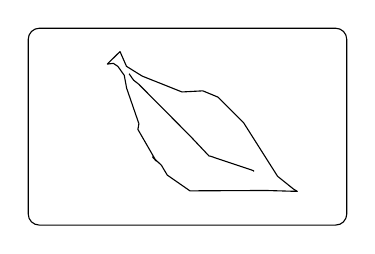
\begin{tikzpicture}[scale=.5]
 \pgfmathsetmacro\gr{1.61803}
      \pgfmathsetmacro\by{5pt}
      \pgfmathsetmacro\bx{\by*\gr}
      \draw[rounded corners] (0,0) rectangle (\bx,\by);

      \pgfmathsetmacro\wx{1.25pt}
      \pgfmathsetmacro\wy{1.25pt}

       \draw [line join=round] (\wx * 2, \wy * 2.78) -- ++(100.52:9.493pt) -- ++(125.31:7.843pt) -- ++(145.78:4.031pt) -- ++(-173.09:4.432pt) -- ++(44.58:12.917pt) -- ++(-66.37:11.643pt) -- ++(-31.94:13.356pt) -- ++(-21.71:30.999pt) -- ++(3.04:15.088pt) -- ++(-22.52:11.836pt) -- ++(-45.00:26.210pt) -- ++(-57.61:45.793pt) -- ++(-38.74:14.701pt) -- ++(-31.76:3.293pt) -- ++(178.32:22.676pt) -- ++(-179.72:54.934pt) -- ++(145.20:19.950pt) -- ++(120.74:8.3pt) -- ++(136.85:8.773pt) -- (\wx * 2.6, \wy * 1.3) -- ++(120:26.43pt) -- ++(80:4.21pt) -- cycle;

      \draw [line join=round] (\wx * 2.05, \wy * 3.075) -- ++(-55.18:5.604pt) -- ++(-38.29:4.841pt) -- (\wx * 3.3, \wy * 1.8) -- ++(-46.66:19.524pt) -- (\wx * 3.7, \wy * 1.4) -- ++(-18.55:32.698pt) -- ++(-45.00:.849pt);
    \end{tikzpicture}
    \caption{End \dots}
  \end{subfigure}
  \hfill
  \begin{subfigure}[h]{0.4\linewidth}
    \centering
  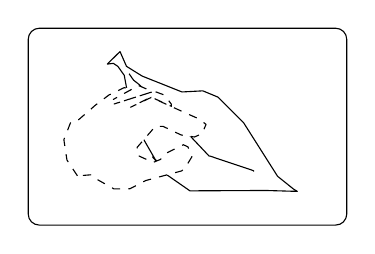
\begin{tikzpicture}[scale=.5]
    \pgfmathsetmacro\gr{1.61803}
    \pgfmathsetmacro\by{5pt}
    \pgfmathsetmacro\bx{\by*\gr}
    \draw[rounded corners] (0,0) rectangle (\bx,\by);

    \pgfmathsetmacro\wx{1.25pt}
    \pgfmathsetmacro\wy{1.25pt}

    \draw [line join=round] (\wx * 2, \wy * 2.78) -- ++(100.52:9.493pt) -- ++(125.31:7.843pt) -- ++(145.78:4.031pt) -- ++(-173.09:4.432pt) -- ++(44.58:12.917pt) -- ++(-66.37:11.643pt) -- ++(-31.94:13.356pt) -- ++(-21.71:30.999pt) -- ++(3.04:15.088pt) -- ++(-22.52:11.836pt) -- ++(-45.00:26.210pt) -- ++(-57.61:45.793pt) -- ++(-38.74:14.701pt) -- ++(-31.76:3.293pt) -- ++(178.32:22.676pt) -- ++(-179.72:54.934pt) -- ++(145.20:19.950pt) -- ++(120.74:8.3pt) -- ++(136.85:8.773pt) -- (\wx * 2.6, \wy * 1.3) -- ++(120:26.43pt) -- ++(80:4.21pt) -- cycle;

    \draw [line join=round] (\wx * 2.05, \wy * 3.075) -- ++(-55.18:5.604pt) -- ++(-38.29:4.841pt) -- (\wx * 3.3, \wy * 1.8) -- ++(-46.66:19.524pt) -- (\wx * 3.7, \wy * 1.4) -- ++(-18.55:32.698pt) -- ++(-45.00:.849pt);

    \draw [line join=round, dashed, fill=white] (\wx,\wy) -- ++(123.46:13.784pt) -- ++(98.57:14.864pt) -- ++(68.43:13.872pt) -- ++(15:5.797pt) -- ++(40.95:16.021pt) -- ++(36.96:12.140pt) -- ++(25.73:12.210pt) -- ++(-6.34:6.339pt) -- ++(-151.16:16.059pt) -- ++(28.65:20.854pt)-- ++(-23.13:11.200pt) -- ++(-162.37:29.380pt) -- ++(17.66:30.329pt) -- ++(-20.22:8.099pt) -- ++(-53.56:8.080pt) -- ++(-86.42:1.603pt) -- ++(155.50:16.155pt) -- ++(-153.67:16.595pt) -- ++(25.33:16.595pt) -- ++(-24.50:16.155pt) -- ++(-24.10:21.800pt) -- ++(-37.95:6.341pt) -- ++(-113.40:7.301pt) -- ++(-156.43:6.001pt) -- ++(171.21:9.815pt) -- ++(154.50:14.403pt) -- ++(-177.99:5.704pt) -- ++(-130.91:19.849pt) -- ++(-86.05:5.814pt) -- ++(-24.68:12.216pt) -- ++(22.17:5.831pt) -- ++(43.90:7.355pt) -- ++(26.15:12.478pt) -- ++(-24.44:3.625pt) -- ++(-68.20:7.739pt) -- ++(-121.18:8.884pt) -- ++(-136.08:3.748pt) -- ++(-164.99:27.022pt) -- ++(-152.43:12.748pt) -- ++(-179.51:11.700pt) -- ++(150.58:15.269pt) -- ++(136.04:3.890pt) -- cycle;
    \end{tikzpicture}
    \caption{\dots and means}
  \end{subfigure}
  \hfill\mbox{}
  \caption{Ends and means in logical space}
  \label{tikz:MEprinciple:setup}
\end{figure}


For example, the act of obtaining an ingredient is identified with the proposition in which the ingredient is obtained, which may be a means to the end of using the ingredient, which is the set of worlds in the ingredient is used, or the proposition that the ingredient is used.

If the set of worlds in which the ingredient is obtained is included in the set of worlds in which the ingredient is used, then obtaining the ingredient is a sufficient means to the end of using the ingredient, though it may not be necessary.\nolinebreak
\footnote{Homework exercise.}

And, conversely, if the set of worlds in the ingredient is used is a subset of the worlds in which the ingredient is obtained, then obtaining the ingredient is a necessary but not necessarily sufficient means to using the ingredient.\nolinebreak
\footnote{This one is much easier.}
This is illustrated in figure~\ref{tikz:MEprinciple:setup}.

Notice that the notions of necessity and sufficiency of means to ends is explained by what is true at certain worlds:
Obtaining the ingredient is a means to the end of using the ingredient because there is a world in which you are have obtained the ingredient and have used the ingredient.
That is, there's little more to means-end relations that coincidence of truth at a world.

This is illustrated in figure~\ref{tikz:MEprinciple:possibility}.

\begin{figure}[ht]
  \hfill
  \begin{subfigure}[h]{0.4\linewidth}
    \centering
  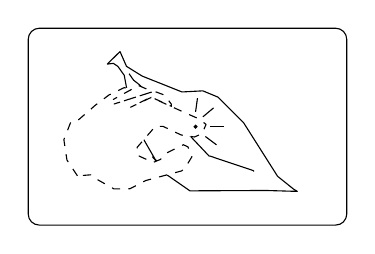
\begin{tikzpicture}[scale=.5]
    \pgfmathsetmacro\gr{1.61803}
    \pgfmathsetmacro\by{5pt}
    \pgfmathsetmacro\bx{\by*\gr}
    \draw[rounded corners] (0,0) rectangle (\bx,\by);

    \pgfmathsetmacro\wx{1.25pt}
    \pgfmathsetmacro\wy{1.25pt}

    \draw [line join=round] (\wx * 2, \wy * 2.78) -- ++(100.52:9.493pt) -- ++(125.31:7.843pt) -- ++(145.78:4.031pt) -- ++(-173.09:4.432pt) -- ++(44.58:12.917pt) -- ++(-66.37:11.643pt) -- ++(-31.94:13.356pt) -- ++(-21.71:30.999pt) -- ++(3.04:15.088pt) -- ++(-22.52:11.836pt) -- ++(-45.00:26.210pt) -- ++(-57.61:45.793pt) -- ++(-38.74:14.701pt) -- ++(-31.76:3.293pt) -- ++(178.32:22.676pt) -- ++(-179.72:54.934pt) -- ++(145.20:19.950pt) -- ++(120.74:8.3pt) -- ++(136.85:8.773pt) -- (\wx * 2.6, \wy * 1.3) -- ++(120:26.43pt) -- ++(80:4.21pt) -- cycle;

    \draw [line join=round] (\wx * 2.05, \wy * 3.075) -- ++(-55.18:5.604pt) -- ++(-38.29:4.841pt) -- (\wx * 3.3, \wy * 1.8) -- ++(-46.66:19.524pt) -- (\wx * 3.7, \wy * 1.4) -- ++(-18.55:32.698pt) -- ++(-45.00:.849pt);

    \draw [line join=round, dashed, fill=white] (\wx,\wy) -- ++(123.46:13.784pt) -- ++(98.57:14.864pt) -- ++(68.43:13.872pt) -- ++(15:5.797pt) -- ++(40.95:16.021pt) -- ++(36.96:12.140pt) -- ++(25.73:12.210pt) -- ++(-6.34:6.339pt) -- ++(-151.16:16.059pt) -- ++(28.65:20.854pt)-- ++(-23.13:11.200pt) -- ++(-162.37:29.380pt) -- ++(17.66:30.329pt) -- ++(-20.22:8.099pt) -- ++(-53.56:8.080pt) -- ++(-86.42:1.603pt) -- ++(155.50:16.155pt) -- ++(-153.67:16.595pt) -- ++(25.33:16.595pt) -- ++(-24.50:16.155pt) -- ++(-24.10:21.800pt) -- ++(-37.95:6.341pt) -- ++(-113.40:7.301pt) -- ++(-156.43:6.001pt) -- ++(171.21:9.815pt) -- ++(154.50:14.403pt) -- ++(-177.99:5.704pt) -- ++(-130.91:19.849pt) -- ++(-86.05:5.814pt) -- ++(-24.68:12.216pt) -- ++(22.17:5.831pt) -- ++(43.90:7.355pt) -- ++(26.15:12.478pt) -- ++(-24.44:3.625pt) -- ++(-68.20:7.739pt) -- ++(-121.18:8.884pt) -- ++(-136.08:3.748pt) -- ++(-164.99:27.022pt) -- ++(-152.43:12.748pt) -- ++(-179.51:11.700pt) -- ++(150.58:15.269pt) -- ++(136.04:3.890pt) -- cycle;

    \draw [fill=black] (\wx * 3.4, \wy * 2) circle (1pt);

    \draw [line join=round, fill=black] (\wx * 3.7, \wy * 2) -- ++(0:10pt);
    \draw [line join=round, fill=black] (\wx * 3.55, \wy * 2.2) -- ++(40:10pt);
    \draw [line join=round, fill=black] (\wx * 3.4, \wy * 2.3) -- ++(82:10pt);
    \draw [line join=round, fill=black] (\wx * 3.6, \wy * 1.8) -- ++(-37:10pt);
    \end{tikzpicture}
    \caption{Possible world \dots}
  \end{subfigure}
  \hfill
  \begin{subfigure}[h]{0.4\linewidth}
    \centering
    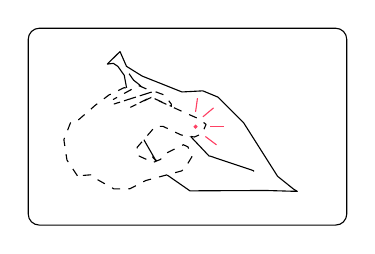
\begin{tikzpicture}[scale=.5]
      \pgfmathsetmacro\gr{1.61803}
      \pgfmathsetmacro\by{5pt}
      \pgfmathsetmacro\bx{\by*\gr}
      \draw[rounded corners] (0,0) rectangle (\bx,\by);

      \pgfmathsetmacro\wx{1.25pt}
      \pgfmathsetmacro\wy{1.25pt}

      \draw [line join=round] (\wx * 2, \wy * 2.78) -- ++(100.52:9.493pt) -- ++(125.31:7.843pt) -- ++(145.78:4.031pt) -- ++(-173.09:4.432pt) -- ++(44.58:12.917pt) -- ++(-66.37:11.643pt) -- ++(-31.94:13.356pt) -- ++(-21.71:30.999pt) -- ++(3.04:15.088pt) -- ++(-22.52:11.836pt) -- ++(-45.00:26.210pt) -- ++(-57.61:45.793pt) -- ++(-38.74:14.701pt) -- ++(-31.76:3.293pt) -- ++(178.32:22.676pt) -- ++(-179.72:54.934pt) -- ++(145.20:19.950pt) -- ++(120.74:8.3pt) -- ++(136.85:8.773pt) -- (\wx * 2.6, \wy * 1.3) -- ++(120:26.43pt) -- ++(80:4.21pt) -- cycle;

      \draw [line join=round] (\wx * 2.05, \wy * 3.075) -- ++(-55.18:5.604pt) -- ++(-38.29:4.841pt) -- (\wx * 3.3, \wy * 1.8) -- ++(-46.66:19.524pt) -- (\wx * 3.7, \wy * 1.4) -- ++(-18.55:32.698pt) -- ++(-45.00:.849pt);

      \draw [line join=round, dashed, fill=white] (\wx,\wy) -- ++(123.46:13.784pt) -- ++(98.57:14.864pt) -- ++(68.43:13.872pt) -- ++(15:5.797pt) -- ++(40.95:16.021pt) -- ++(36.96:12.140pt) -- ++(25.73:12.210pt) -- ++(-6.34:6.339pt) -- ++(-151.16:16.059pt) -- ++(28.65:20.854pt)-- ++(-23.13:11.200pt) -- ++(-162.37:29.380pt) -- ++(17.66:30.329pt) -- ++(-20.22:8.099pt) -- ++(-53.56:8.080pt) -- ++(-86.42:1.603pt) -- ++(155.50:16.155pt) -- ++(-153.67:16.595pt) -- ++(25.33:16.595pt) -- ++(-24.50:16.155pt) -- ++(-24.10:21.800pt) -- ++(-37.95:6.341pt) -- ++(-113.40:7.301pt) -- ++(-156.43:6.001pt) -- ++(171.21:9.815pt) -- ++(154.50:14.403pt) -- ++(-177.99:5.704pt) -- ++(-130.91:19.849pt) -- ++(-86.05:5.814pt) -- ++(-24.68:12.216pt) -- ++(22.17:5.831pt) -- ++(43.90:7.355pt) -- ++(26.15:12.478pt) -- ++(-24.44:3.625pt) -- ++(-68.20:7.739pt) -- ++(-121.18:8.884pt) -- ++(-136.08:3.748pt) -- ++(-164.99:27.022pt) -- ++(-152.43:12.748pt) -- ++(-179.51:11.700pt) -- ++(150.58:15.269pt) -- ++(136.04:3.890pt) -- cycle;

      \draw [fill=fuchsia, color=fuchsia] (\wx * 3.4, \wy * 2) circle (1pt);

      \draw [line join=round, fill=fuchsia, color=fuchsia] (\wx * 3.7, \wy * 2) -- ++(0:10pt);
      \draw [line join=round, fill=fuchsia, color=fuchsia] (\wx * 3.55, \wy * 2.2) -- ++(40:10pt);
      \draw [line join=round, fill=fuchsia, color=fuchsia] (\wx * 3.4, \wy * 2.3) -- ++(82:10pt);
      \draw [line join=round, fill=fuchsia, color=fuchsia] (\wx * 3.6, \wy * 1.8) -- ++(-37:10pt);
    \end{tikzpicture}
  \caption{\dots is possible so \dots}
  \label{fig:supermarket:ex}
\end{subfigure}
\hfill\mbox{}

\hfill
\begin{subfigure}[h]{0.4\linewidth}
  \centering
  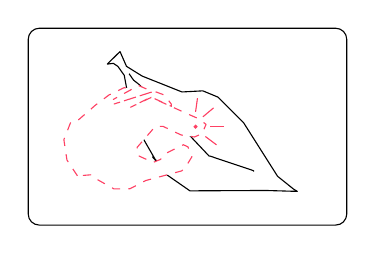
\begin{tikzpicture}[scale=.5]
    \pgfmathsetmacro\gr{1.61803}
    \pgfmathsetmacro\by{5pt}
    \pgfmathsetmacro\bx{\by*\gr}
    \draw[rounded corners] (0,0) rectangle (\bx,\by);

    \pgfmathsetmacro\wx{1.25pt}
    \pgfmathsetmacro\wy{1.25pt}

    \draw [line join=round] (\wx * 2, \wy * 2.78) -- ++(100.52:9.493pt) -- ++(125.31:7.843pt) -- ++(145.78:4.031pt) -- ++(-173.09:4.432pt) -- ++(44.58:12.917pt) -- ++(-66.37:11.643pt) -- ++(-31.94:13.356pt) -- ++(-21.71:30.999pt) -- ++(3.04:15.088pt) -- ++(-22.52:11.836pt) -- ++(-45.00:26.210pt) -- ++(-57.61:45.793pt) -- ++(-38.74:14.701pt) -- ++(-31.76:3.293pt) -- ++(178.32:22.676pt) -- ++(-179.72:54.934pt) -- ++(145.20:19.950pt) -- ++(120.74:8.3pt) -- ++(136.85:8.773pt) -- (\wx * 2.6, \wy * 1.3) -- ++(120:26.43pt) -- ++(80:4.21pt) -- cycle;

    \draw [line join=round] (\wx * 2.05, \wy * 3.075) -- ++(-55.18:5.604pt) -- ++(-38.29:4.841pt) -- (\wx * 3.3, \wy * 1.8) -- ++(-46.66:19.524pt) -- (\wx * 3.7, \wy * 1.4) -- ++(-18.55:32.698pt) -- ++(-45.00:.849pt);

    \draw [line join=round, dashed, color=fuchsia, fill=white] (\wx,\wy) -- ++(123.46:13.784pt) -- ++(98.57:14.864pt) -- ++(68.43:13.872pt) -- ++(15:5.797pt) -- ++(40.95:16.021pt) -- ++(36.96:12.140pt) -- ++(25.73:12.210pt) -- ++(-6.34:6.339pt) -- ++(-151.16:16.059pt) -- ++(28.65:20.854pt)-- ++(-23.13:11.200pt) -- ++(-162.37:29.380pt) -- ++(17.66:30.329pt) -- ++(-20.22:8.099pt) -- ++(-53.56:8.080pt) -- ++(-86.42:1.603pt) -- ++(155.50:16.155pt) -- ++(-153.67:16.595pt) -- ++(25.33:16.595pt) -- ++(-24.50:16.155pt) -- ++(-24.10:21.800pt) -- ++(-37.95:6.341pt) -- ++(-113.40:7.301pt) -- ++(-156.43:6.001pt) -- ++(171.21:9.815pt) -- ++(154.50:14.403pt) -- ++(-177.99:5.704pt) -- ++(-130.91:19.849pt) -- ++(-86.05:5.814pt) -- ++(-24.68:12.216pt) -- ++(22.17:5.831pt) -- ++(43.90:7.355pt) -- ++(26.15:12.478pt) -- ++(-24.44:3.625pt) -- ++(-68.20:7.739pt) -- ++(-121.18:8.884pt) -- ++(-136.08:3.748pt) -- ++(-164.99:27.022pt) -- ++(-152.43:12.748pt) -- ++(-179.51:11.700pt) -- ++(150.58:15.269pt) -- ++(136.04:3.890pt) -- cycle;

    \draw [fill=fuchsia, color=fuchsia] (\wx * 3.4, \wy * 2) circle (1pt);

    \draw [line join=round, fill=fuchsia, color=fuchsia] (\wx * 3.7, \wy * 2) -- ++(0:10pt);
    \draw [line join=round, fill=fuchsia, color=fuchsia] (\wx * 3.55, \wy * 2.2) -- ++(40:10pt);
    \draw [line join=round, fill=fuchsia, color=fuchsia] (\wx * 3.4, \wy * 2.3) -- ++(82:10pt);
    \draw [line join=round, fill=fuchsia, color=fuchsia] (\wx * 3.6, \wy * 1.8) -- ++(-37:10pt);
    \end{tikzpicture}
  \caption{\dots means is possible and \dots}
  \label{fig:supermarket:ex}
\end{subfigure}
\hfill
\begin{subfigure}[h]{0.4\linewidth}
  \centering
  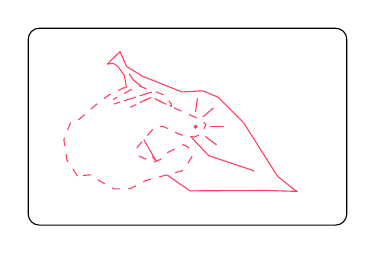
\begin{tikzpicture}[scale=.5]
    \pgfmathsetmacro\gr{1.61803}
    \pgfmathsetmacro\by{5pt}
    \pgfmathsetmacro\bx{\by*\gr}
    \draw[rounded corners] (0,0) rectangle (\bx,\by);

    \pgfmathsetmacro\wx{1.25pt}
    \pgfmathsetmacro\wy{1.25pt}

    \draw [line join=round, color=fuchsia] (\wx * 2, \wy * 2.78) -- ++(100.52:9.493pt) -- ++(125.31:7.843pt) -- ++(145.78:4.031pt) -- ++(-173.09:4.432pt) -- ++(44.58:12.917pt) -- ++(-66.37:11.643pt) -- ++(-31.94:13.356pt) -- ++(-21.71:30.999pt) -- ++(3.04:15.088pt) -- ++(-22.52:11.836pt) -- ++(-45.00:26.210pt) -- ++(-57.61:45.793pt) -- ++(-38.74:14.701pt) -- ++(-31.76:3.293pt) -- ++(178.32:22.676pt) -- ++(-179.72:54.934pt) -- ++(145.20:19.950pt) -- ++(120.74:8.3pt) -- ++(136.85:8.773pt) -- (\wx * 2.6, \wy * 1.3) -- ++(120:26.43pt) -- ++(80:4.21pt) -- cycle;

    \draw [line join=round, color=fuchsia] (\wx * 2.05, \wy * 3.075) -- ++(-55.18:5.604pt) -- ++(-38.29:4.841pt) -- (\wx * 3.3, \wy * 1.8) -- ++(-46.66:19.524pt) -- (\wx * 3.7, \wy * 1.4) -- ++(-18.55:32.698pt) -- ++(-45.00:.849pt);

    \draw [line join=round, dashed, color=fuchsia, fill=white] (\wx,\wy) -- ++(123.46:13.784pt) -- ++(98.57:14.864pt) -- ++(68.43:13.872pt) -- ++(15:5.797pt) -- ++(40.95:16.021pt) -- ++(36.96:12.140pt) -- ++(25.73:12.210pt) -- ++(-6.34:6.339pt) -- ++(-151.16:16.059pt) -- ++(28.65:20.854pt)-- ++(-23.13:11.200pt) -- ++(-162.37:29.380pt) -- ++(17.66:30.329pt) -- ++(-20.22:8.099pt) -- ++(-53.56:8.080pt) -- ++(-86.42:1.603pt) -- ++(155.50:16.155pt) -- ++(-153.67:16.595pt) -- ++(25.33:16.595pt) -- ++(-24.50:16.155pt) -- ++(-24.10:21.800pt) -- ++(-37.95:6.341pt) -- ++(-113.40:7.301pt) -- ++(-156.43:6.001pt) -- ++(171.21:9.815pt) -- ++(154.50:14.403pt) -- ++(-177.99:5.704pt) -- ++(-130.91:19.849pt) -- ++(-86.05:5.814pt) -- ++(-24.68:12.216pt) -- ++(22.17:5.831pt) -- ++(43.90:7.355pt) -- ++(26.15:12.478pt) -- ++(-24.44:3.625pt) -- ++(-68.20:7.739pt) -- ++(-121.18:8.884pt) -- ++(-136.08:3.748pt) -- ++(-164.99:27.022pt) -- ++(-152.43:12.748pt) -- ++(-179.51:11.700pt) -- ++(150.58:15.269pt) -- ++(136.04:3.890pt) -- cycle;

    \draw [fill=fuchsia, color=fuchsia] (\wx * 3.4, \wy * 2) circle (1pt);

    \draw [line join=round, fill=fuchsia, color=fuchsia] (\wx * 3.7, \wy * 2) -- ++(0:10pt);
    \draw [line join=round, fill=fuchsia, color=fuchsia] (\wx * 3.55, \wy * 2.2) -- ++(40:10pt);
    \draw [line join=round, fill=fuchsia, color=fuchsia] (\wx * 3.4, \wy * 2.3) -- ++(82:10pt);
    \draw [line join=round, fill=fuchsia, color=fuchsia] (\wx * 3.6, \wy * 1.8) -- ++(-37:10pt);
    \end{tikzpicture}
  \caption{\dots end is possible.}
  \label{fig:supermarket:ex}
\end{subfigure}
\hfill\mbox{}
\caption{Example of principle~\ref{princple:dependence} wrt.\ evaluations of possibility.}
\label{tikz:MEprinciple:possibility}
\end{figure}


Now, an agent's evaluation of obtaining an ingredient as worthwhile is an evaluation of some set of worlds as worthwhile, and depending on the overlap between those worlds in which the agent has obtained the ingredient and has used the ingredient, obtaining the ingredient will likewise be evaluated as worthwhile.
This is illustrated in figure~\ref{tikz:MEprinciple:worthwhile}.

\begin{figure}[ht]
  \hfill
\begin{subfigure}[h]{0.4\linewidth}
  \centering
  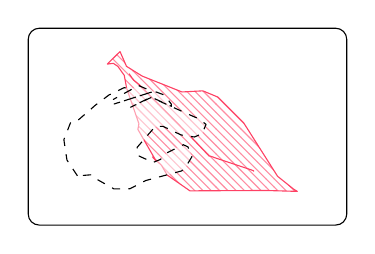
\begin{tikzpicture}[scale=.5]
    \pgfmathsetmacro\gr{1.61803}
    \pgfmathsetmacro\by{5pt}
    \pgfmathsetmacro\bx{\by*\gr}
    \draw[rounded corners] (0,0) rectangle (\bx,\by);

    \pgfmathsetmacro\wx{1.25pt}
    \pgfmathsetmacro\wy{1.25pt}

    \draw [line join=round, color=fuchsia, pattern=north west lines, pattern color=fuchsia!60] (\wx * 2, \wy * 2.78) -- ++(100.52:9.493pt) -- ++(125.31:7.843pt) -- ++(145.78:4.031pt) -- ++(-173.09:4.432pt) -- ++(44.58:12.917pt) -- ++(-66.37:11.643pt) -- ++(-31.94:13.356pt) -- ++(-21.71:30.999pt) -- ++(3.04:15.088pt) -- ++(-22.52:11.836pt) -- ++(-45.00:26.210pt) -- ++(-57.61:45.793pt) -- ++(-38.74:14.701pt) -- ++(-31.76:3.293pt) -- ++(178.32:22.676pt) -- ++(-179.72:54.934pt) -- ++(145.20:19.950pt) -- ++(120.74:8.3pt) -- ++(136.85:8.773pt) -- (\wx * 2.6, \wy * 1.3) -- ++(120:26.43pt) -- ++(80:4.21pt) -- cycle;

    \draw [line join=round, color=fuchsia, fill opacity=0.5] (\wx * 2.05, \wy * 3.075) -- ++(-55.18:5.604pt) -- ++(-38.29:4.841pt) -- (\wx * 3.3, \wy * 1.8) -- ++(-46.66:19.524pt) -- (\wx * 3.7, \wy * 1.4) -- ++(-18.55:32.698pt) -- ++(-45.00:.849pt);

    \draw [line join=round, dashed, fill=white, fill opacity=0.5] (\wx,\wy) -- ++(123.46:13.784pt) -- ++(98.57:14.864pt) -- ++(68.43:13.872pt) -- ++(15:5.797pt) -- ++(40.95:16.021pt) -- ++(36.96:12.140pt) -- ++(25.73:12.210pt) -- ++(-6.34:6.339pt) -- ++(-151.16:16.059pt) -- ++(28.65:20.854pt)-- ++(-23.13:11.200pt) -- ++(-162.37:29.380pt) -- ++(17.66:30.329pt) -- ++(-20.22:8.099pt) -- ++(-53.56:8.080pt) -- ++(-86.42:1.603pt) -- ++(155.50:16.155pt) -- ++(-153.67:16.595pt) -- ++(25.33:16.595pt) -- ++(-24.50:16.155pt) -- ++(-24.10:21.800pt) -- ++(-37.95:6.341pt) -- ++(-113.40:7.301pt) -- ++(-156.43:6.001pt) -- ++(171.21:9.815pt) -- ++(154.50:14.403pt) -- ++(-177.99:5.704pt) -- ++(-130.91:19.849pt) -- ++(-86.05:5.814pt) -- ++(-24.68:12.216pt) -- ++(22.17:5.831pt) -- ++(43.90:7.355pt) -- ++(26.15:12.478pt) -- ++(-24.44:3.625pt) -- ++(-68.20:7.739pt) -- ++(-121.18:8.884pt) -- ++(-136.08:3.748pt) -- ++(-164.99:27.022pt) -- ++(-152.43:12.748pt) -- ++(-179.51:11.700pt) -- ++(150.58:15.269pt) -- ++(136.04:3.890pt) -- cycle;
    \end{tikzpicture}
  \caption{Worthwhile end so \dots}
  \label{fig:supermarket:ex}
\end{subfigure}
\hfill
\begin{subfigure}[h]{0.4\linewidth}
  \centering  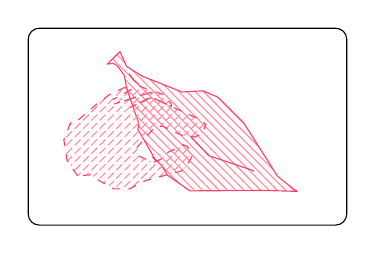
\begin{tikzpicture}[scale=.5]
    \pgfmathsetmacro\gr{1.61803}
    \pgfmathsetmacro\by{5pt}
    \pgfmathsetmacro\bx{\by*\gr}
    \draw[rounded corners] (0,0) rectangle (\bx,\by);

    \pgfmathsetmacro\wx{1.25pt}
    \pgfmathsetmacro\wy{1.25pt}

   \draw [line join=round, color=fuchsia, fill=white, fill opacity=0.5, pattern=north west lines, pattern color=fuchsia!60] (\wx * 2, \wy * 2.78) -- ++(100.52:9.493pt) -- ++(125.31:7.843pt) -- ++(145.78:4.031pt) -- ++(-173.09:4.432pt) -- ++(44.58:12.917pt) -- ++(-66.37:11.643pt) -- ++(-31.94:13.356pt) -- ++(-21.71:30.999pt) -- ++(3.04:15.088pt) -- ++(-22.52:11.836pt) -- ++(-45.00:26.210pt) -- ++(-57.61:45.793pt) -- ++(-38.74:14.701pt) -- ++(-31.76:3.293pt) -- ++(178.32:22.676pt) -- ++(-179.72:54.934pt) -- ++(145.20:19.950pt) -- ++(120.74:8.3pt) -- ++(136.85:8.773pt) -- (\wx * 2.6, \wy * 1.3) -- ++(120:26.43pt) -- ++(80:4.21pt) -- cycle;

    \draw [line join=round, color=fuchsia, fill=fuchsia!60] (\wx * 2.05, \wy * 3.075) -- ++(-55.18:5.604pt) -- ++(-38.29:4.841pt);

    \draw [line join=round, color=fuchsia, fill=fuchsia!60] (\wx * 3.3, \wy * 1.8) -- ++(-46.66:19.524pt);

    \draw [line join=round, color=fuchsia, fill=fuchsia!60] (\wx * 3.7, \wy * 1.4) -- ++(-18.55:32.698pt) -- ++(-45.00:.849pt);

    \draw [line join=round, dashed, color=fuchsia, pattern=north east lines, pattern color=fuchsia!60] (\wx,\wy) -- ++(123.46:13.784pt) -- ++(98.57:14.864pt) -- ++(68.43:13.872pt) -- ++(15:5.797pt) -- ++(40.95:16.021pt) -- ++(36.96:12.140pt) -- ++(25.73:12.210pt) -- ++(-6.34:6.339pt) -- ++(-151.16:16.059pt) -- ++(28.65:20.854pt)-- ++(-23.13:11.200pt) -- ++(-162.37:29.380pt) -- ++(17.66:30.329pt) -- ++(-20.22:8.099pt) -- ++(-53.56:8.080pt) -- ++(-86.42:1.603pt) -- ++(155.50:16.155pt) -- ++(-153.67:16.595pt) -- ++(25.33:16.595pt) -- ++(-24.50:16.155pt) -- ++(-24.10:21.800pt) -- ++(-37.95:6.341pt) -- ++(-113.40:7.301pt) -- ++(-156.43:6.001pt) -- ++(171.21:9.815pt) -- ++(154.50:14.403pt) -- ++(-177.99:5.704pt) -- ++(-130.91:19.849pt) -- ++(-86.05:5.814pt) -- ++(-24.68:12.216pt) -- ++(22.17:5.831pt) -- ++(43.90:7.355pt) -- ++(26.15:12.478pt) -- ++(-24.44:3.625pt) -- ++(-68.20:7.739pt) -- ++(-121.18:8.884pt) -- ++(-136.08:3.748pt) -- ++(-164.99:27.022pt) -- ++(-152.43:12.748pt) -- ++(-179.51:11.700pt) -- ++(150.58:15.269pt) -- ++(136.04:3.890pt) -- cycle;
    \end{tikzpicture}
  \caption{\dots worthwhile means.}
  \label{fig:supermarket:ex}
\end{subfigure}
\hfill\mbox{}
\caption{Example of principle~\ref{princple:dependence} wrt.\ evaluations of worthwhileness.}
\label{tikz:MEprinciple:worthwhile}
\end{figure}

% \citeauthor{Jeffrey:1990aa}-style example to illustrate the gist of the principle.

% Standard point semantics for propositional logic.
% Relation between \(P\) and \(Q\).
% If \(P\) is true, \(Q\) must be true.
% This generalises.
% Possible worlds, truth, and a probabiltiy distribution.
% Follow \citeauthor{Jeffrey:1990aa} and ideftify acts with outcomes.
% Add in an additional function for what is worthwhile, and now we have an instance of principle~\ref{princple:dependence}.
% A few more assumptions will get us something like \citeauthor{Jeffrey:1990aa}'s decision theory, and some worries about gunk will force a revision,

\newpage

\hozline

\subsection*{Everyone agrees that something \emph{like} the principle is a \emph{good thing}}
\label{sec:everyone-agrees-that}

\hozline

\subsubsection*{Kant}
\label{sec:kant}

\citeauthor{Kant:1948aa} in \citetitle{Kant:1948aa} states:\nolinebreak
\footnote{\citeauthor{Kant:1948aa} took this to be analytic:
  \begin{quote}
    So far as willing is concerned, this proposition is analytic: for in my willing of an object as an effect there is already conceived the causality of myself as an acting cause---that is, the use of means; and from the concept of willing an end the imperative merely extracts the concept of actions necessary to this end.\nolinebreak
    \mbox{ }\hfill(\citeyear[81]{Kant:1948aa})
  \end{quote}
  The argument is a mystery to me\dots

  Alternative translation:
\begin{quote}
  Whoever wills the end also wills (insofar as reason has decisive influence on his actions) the indispensably necessary means to it that are within his power.

  This proposition is, as regards the volition, analytic; for in the volition of an object as my effect, my causality as acting cause, that is, the use of means, is already thought, and the imperative extracts the concept of actions necessary to this end merely from the concept of a volition of this end\dots\nolinebreak
  \mbox{ }\hfill(\citeyear[28]{Kant:1997aa})
\end{quote}
}

\begin{quote}
  Who wills the end, wills (so far as reason has a decisive influence on his actions) also the means which are indispensably necessary and in his power.\nolinebreak
  \mbox{ }\hfill\mbox{(\citeyear[80--81/Ak 417]{Kant:1948aa})}
\end{quote}


\hozline

\subsubsection*{Hume}
\label{sec:hume}

\citeauthor{Hume:2011aa} in \citetitle{Hume:2011aa} writes:

\begin{quote}
  I may will the performance of certain actions as means of obtaining any desired good; but as my willing of these actions is only secondary, and founded on the supposition, that they are causes of the proposed effect; as soon as I discover the falshood of that supposition, they must become indifferent to me.\nolinebreak
  \mbox{ }\hfill\mbox{\hfill(T2.3.3)}
\end{quote}

\hozlinedash

Similarly, \citeauthor{Sinhababu:2017aa}, defending a Humean theory of practical reasoning --- rather than \citeauthor{Hume:2011aa}'s theory of practical reasoning --- writes:

\begin{quote}
  The Motivational Aspect:
  Desire that E combined with belief that one could increase E's probability by A-ing motivates one to A, proportional to the desire's strength times the increase in subjective probability of E.
  (With belief that A-ing would reduce E's probability, it likewise motivates one not to A.)\nolinebreak
  \mbox{ }\hfill\mbox{(\citeyear[23]{Sinhababu:2017aa})}
\end{quote}

\hozline

\subsubsection*{Differences between Kant and Hume \hfill (Green Beans with Cherry Tomatoes)}
\label{sec:role-reason}



As \citeauthor{Dreier:2001aa} highlights, the parenthetical use of reason in \citeauthor{Kant:1948aa}'s formulation is quite useful as it allows one to understand an agent that desires to \(\psi\), believe that by \(\phi\)-ing they will \(\psi\), and yet fails to desire to \(\phi\) as irrational rather than impossible (\citeyear[35]{Dreier:2001aa}).

Perhaps the `must' in \citeauthor{Hume:2011aa}'s principle can be read in terms of reason, but more likely it is that of necessity.
For example, while \citeauthor{Sinhababu:2017aa} seems to leave no doubt.

Perhaps an agent is irrational if they fail to will or desire the means to the ends they, likewise, will or desire.
Or, perhaps an agent who fails to do so in turns fails to have beliefs or desires in some appropriately strict sense.
Either way, the relation between ends and means is clear.

\hozlinedash

\citeauthor{Kant:1948aa} and \citeauthor{Hume:2011aa} also differ by taking about `willing' and `desiring', respectively.
I don't think this is too important.
If `willing' is like `intending' and suggests the selection of an end, then \citeauthor{Kant:1948aa}'s principle may be seen as a special application of a principle like principle~\ref{princple:dependence}.

\hozline


\subsubsection*{Aristotle}\mbox{ }

\citeauthor{Aristotle:2000aa} in book 3 of the \citetitle{Aristotle:2000aa} writes:

\begin{quote}
  We deliberate not about ends, but about things that are conducive to ends.
  For a doctor does not deliberate about whether to cure, nor an orator whether to persuade, nor a politician whether to produce good order; nor does anyone else deliberate about his end. Rather they establish an end and then go on to think about how and by what means it is to be achieved.
  If it appears that there are several means available, they consider by which it will be achieved in the easiest and most noble way; while if it can be attained by only one means, they consider how this will bring it about, and by what further means this means is itself to be brought about, until they arrive at the first cause, the last thing to be found.
  For the person who deliberates seems to inquire and analyse in the way described as though he were dealing with a geometrical figure (it seems that not all inquiry is deliberation --- mathematics, for example --- but that all deliberation is inquiry), and the last step in the analysis seems to be the first that comes to be.

  \dots

  Since the object of rational choice is one of the things in our power that is desired after deliberation, rational choice will be deliberative desire for things in our power; for, when we have decided on the basis of deliberation, we desire in accordance with our deliberation.\nolinebreak
  \mbox{ }\hfill\mbox{(III.3, 1112b--1113a)}
\end{quote}

`Desired after deliberation' \dots, does this mean that a desire is formed, or that the means is seen as a way to the end?

\newpage

\hozline

\subsubsection*{Nagel \hfill (Candied Yams)\footnote{Parenthetical remark \(\to\) aside \(\to\) a side \(\to\) a side dish.}}
\label{sec:nagel}

\citeauthor{Nagel:1970aa} notes the above passage from \citeauthor{Aristotle:2000aa} when distinguishing motivated from unmotivated desires:

\begin{quote}
  \dots many desires, like many beliefs, are arrived at by decision and after deliberation.
  They need not simply assail us, though there are certain desires that do, like the appetites and in certain cases the emotions.
  The same is true of beliefs, for often, as when we simply perceive something, we acquire a belief without arriving at it by decision.
  The desires which simply come to us are unmotivated though they can be explained.
  Hunger is produced by lack of food, but is not motivated thereby.
  A desire to shop for groceries, after discovering nothing appetizing in the refrigerator, is on the other hand motivated by hunger.
  Rational or motivational explanation is just as much in order for that desire as for the action itself.\nolinebreak
  \mbox{ }\hfill(\citeyear[29]{Nagel:1970aa})
\end{quote}

\citeauthor{Nagel:1970aa}'s account of desire here seems to be in tension with the conclusion of the core argument.
For, if means must be motivated desires then they must be arrived at `by decision and after deliberation'.
However, \citeauthor{Nagel:1970aa} doesn't say this must be deliberation from ends to means, and I only stumbled upon \citetitle{Nagel:1970aa} a few days ago so \dots

\hozline

\subsubsection*{More quotes about means and ends}
\label{sec:more-quotes}


\begin{quote}
    the value of the means derives from the value of the ends \dots
    If there are reasons to take the means, they must be none other than the reasons to pursue the ends, or at least they must derive from them.\nolinebreak
  \mbox{ }\hfill(\cite[2]{Raz:2005aa})
\end{quote}

\begin{quote}
  Consider cases of means-end rationality, that is, cases in which I form a desire to perform the means to an end because I have a background desire for that end and a belief that the means is a means to that end.\linebreak
  \mbox{ }\hfill(\cite[84]{Smith:2004aa})
\end{quote}

\begin{quote}
  Most objectives and activities derive their value from the means-ends relationships which connect them with objectives or activities that are valued in themselves.
  By a process of anticipation, the value inhering in the desired end is transferred to the means.\nolinebreak
  \mbox{ }\hfill(\cite[61]{Simon:1997aa})
\end{quote}

\begin{quote}
  The instrumental value of a means is not to be counted as additional to the intrinsic value of the end.
  (Otherwise, we would be obliged to pursue our ends as circuitously as possible, so as to accumulate the most instrumental value along the way.)
  Since the value of a means is not additional to that of the end, turning a misfortune into a means of learning a lesson doesn’t produce any more value than that inherent in the lesson itself, a value not necessarily greater than that of any alternative lesson one might have learned.\linebreak
  \mbox{ }\hfill(\cite[65]{Velleman:2000ab})
\end{quote}

\begin{quote}
  The ``will'' to attain an end is being transmitted to (use of) the means deemed necessary for its attainment.
  This principle of ``transmission of intention from ends to means'' is basically identical, it seems, with a principle which Kant thought analytically (logically) true and which he expressed in the following words:
  ``Who wills the end, wills (so far as reason has decisive influence on his actions) also the means which are indispensably necessary and in his power.''\nolinebreak
  \mbox{ }\hfill(\cite[40]{Von-Wright:1972aa})
\end{quote}

\begin{quote}
  Reasons are transmitted across the relation between ends and means, and that is also the commonest and simplest way that motivational influence is transmitted.\nolinebreak
  \mbox{ }\hfill(\cite[33]{Nagel:1970aa})
\end{quote}

\begin{quote}
  The solution is to confer a privileged status on the relation between ends and means.
  This is easily incorporated into the definition of a reason.
  We may say that if being thirsty provides a reason to drink, then it also provides a reason for what enables one to drink. That can be regarded as the consequence of a perfectly general property of reasons for action: that they transmit their influence over the relation between ends and means.\nolinebreak
  \mbox{ }\hfill(\cite[34]{Nagel:1970aa})
\end{quote}

\begin{quote}
  But when the fox hath once got in his nose, He’ll soon find means to make the body follow.\newline
  \mbox{ }\hfill\mbox{(\citetitle[4.7.25]{Shakespeare:1968aa})}
\end{quote}

\newpage

\subsection*{Primary Scenario}
\label{sec:scenario}

\hozline

\subsubsection*{Supermarket}

\begin{scenario}\label{scenario:shopping}\footnote{The joke, uh \dots that \dots crikey \dots is that \citeauthor{Anscombe:1957aa}'s shopping list example is \emph{the} example for motivating ideas about direction of fit, but the agent doesn't have the shopping list, which would solve the problem completely as they would be able to see whether the ingredient is a means --- the shopping list, of course, being both the literal and figurative result of their deliberation from the relevant end.}
  Snow dances and random flicker turns to rigid form as the agent regains focus.
  The supermarket aisle is empty, and their left hand is stretched toward an item as if ready to impart life.
  Shucks.
  Forgetting the shopping list, and now forgetting consciousness.
  The agent is in a rough spot.
  And more.
  What were they doing?
  Their outstretched hand suggests they were about to obtain the item.
  No basket, so perhaps this is all they came in for.
  But what would the item be for?
  What is the item a means to?
\end{scenario}

\hozlinedash

Supermarkets are big places and they contain lots of items.
Most of the time people are in supermarkets for food, and most of the time outstretched hands in supermarkets are ready to pick up items.
Suppose for simplicity the agent was reaching for the item as a means, and that this is what they think they were doing.
Whatever the item is, the agent is unable to make sense doing anything with it other than in order to help bring something else about, and their left hand is as unambiguous as a hand can be.
The agent's loss of consciousness conveniently separates their prior practical reasoning and eventual action from their current reasoning and possible action, and the agent's loss of memory concerns the end to the means they were performing when reaching for the item.
The agent has amnesia, but it's the kind of amnesia that amnesia that doesn't need a sophisticated Greek term; it's forgetting and it's mundane.
The agent's loss of consciousness and forgetting of an end combine to interrupt the conclusion of an otherwise unremarkable action.
The issue is whether the agent is able to continue the action?
Are they able to pick up the item as a means to some end?

Picking up the item has a lot going for it.
It is as clear as can be from the agent's outstretched hand that picking up the item once settled what to do, and, it would be strange to infer that the end (whatever it is) is no longer worthwhile because it has been forgotten.
However, because the end has been forgotten the agent cannot reason that picking up the item settles what to do by combining their evaluation of the end as worthwhile with their evaluation of the means as a way to achieve that end.
Instead, the reasoning is inverted:
Because picking up the item settled what to do, some end must have been evaluated as worthwhile and the means as a way to achieve that end.
A proper inversion requires that the recognition that some end was evaluated as worthwhile and a means as a way to achieve that end \emph{settles} picking up the item.
Broadly stated, this kind of reasoning seems impermissible.
That an agent evaluated being healthy as worthwhile and is now jogging as a means to being healthy cannot commit them to perpetual jogging, understood either as a singular activity or a habit.
Whether jogging makes sense depends on whether it helps achieves what the agent evaluates as worthwhile; not what they did.
Yet, forgetting things is not uncommon, and it seems permissible for the agent to pick up the ingredient despite being unable to remember what they would be obtaining the ingredient for.
The agent may worry that they will be unable to remember the end or that they would evaluate it differently to before, but this an item in a supermarket, the stakes don't get much lower.
% More often than not the thought that something \emph{might} be written on my missing shopping list or \emph{maybe would have been} if I had the foresight to think about it is enough to get me thinking, and the realisation that I could need to return to the supermarket .\nolinebreak
% \footnote{Perhaps the agent ate a radioactive radish \dots}

% I start sentences and wonder what I meant to say, stride confidently into rooms only to pace circles looking for the reason, and let an album play as I probably put it on for at least one song and maybe this tedious stuff is an necessary prelude.
Moreover, if the agent settles on obtaining the ingredient it seems they would do so not because it seems they once evaluated some end as worthwhile, but because it seems they still do --- even though they cannot remember what it is.
The agent may take their outstretched hand to provide information that the end they cannot remember is worthwhile, and on this basis pursue means to that end.

The cases of interest involve an agent forgetting the end to some means while either performing or recognising the means as a means to some end.

\hozline

\newpage

\subsubsection*{Structure of scenario and notes}
\label{sec:structure-notes-scenarios}

\hozline

The basic structure of the scenario is:

\begin{enumerate}
\item An agent settles on some end \(e\).
\item The agent engages in means-end reasoning to settle on some means \(m\) to \(e\).
\item The agent loses track of end \(e\) but is able to recall means \(m\).
\item The agent  realises that the means \(m\) is a means to some end, though the agent is unable to recall end \(e\).
\item The agent reasons that as they previously reasoned from some end to means \(m\) that \(e\) is still (maybe subjectively likely to be) worthwhile.
\item So, by principle~\ref{princple:dependence} the means \(m\) is still a candidate for settling what to do.
\item Additional features of the scenario suggest that it is permissible for the agent to continue to pursue means \(m\) (despite being unable to recall end \(e\)).
\item The agent settles on means \(m\).
\end{enumerate}

\hozlinedash

\begin{quote}
  I try to plan, \dots but that isn't my basic mode, really.
  I improvise.
  It’s my greatest talent.
  I prefer situations to plans, you see \dots.

  \mbox{ }\hfill --- Wintermute

  \mbox{ }\hfill\mbox{(\cite[118]{Gibson:2000aa})}
\end{quote}

\hozline

\subsubsection*{Notes}
\label{sec:notes}

\begin{itemize}
\item Instead of settling on \(m\) the agent may do something else.
\item That is, the primary thing of interest is that it is \emph{permissible} for the agent to settle on \(m\).
\item More on this below!
\end{itemize}


\begin{itemize}
\item It is unspecified how far back in the chain of means-end relations the agent is unable to go.
  \begin{itemize}
  \item The agent is unable to recall the specific end \(e\) to which \(m\) is a means, but they may be able to recall some broader end \(e^{+}\) to which \(e\) was a means, and to which \(m\) is also a means.
  \item However, reasoning from \(e^{+}\) to \(m\) would need to require \(e\) (or some other intermediate end).
  \end{itemize}
\end{itemize}

\begin{itemize}
\item What matters is that the agent eventually ends up settles on \(m\) and takes this to be a means to \(e\).
\item The agent may do a whole bunch of reasoning, and some of this reasoning may be used to settle on \(m\), so long as \(m\) is (eventually) taken as a means to some end.
\item For example, the agent may reason about alternative actions that are available to them instead of performing \(m\), and these may help the agent reason about whether performing \(m\) is worthwhile.
\end{itemize}


\begin{itemize}
\item Depending on how you feel about things, the supermarket example may be set up so that the agent either:
  \begin{enumerate}[label=\alph*)]
  \item Reasons from the action that they were (subjectively) likely performing to it being a means to some end, or
  \item is able to directly recall that picking up the item is a means to some end.
  \end{enumerate}
\end{itemize}

\begin{itemize}
\item Due to the means-end structure of the relevant reasoning here, it's not clear that this straightforwardly hooks up to issues about incomplete preferences.
\item For, on my understanding, this primarily concerns how to make evaluative judgements, whereas here it seems as though no explicit evaluative judgement is required --- or is going to be of significant help --- as the appropriate evaluation of the options available to the agent is there, but inaccessible.
\end{itemize}


\newpage

\subsection*{Concerning scenario}
\label{sec:concerning-scenario}

\hozline

\subsubsection*{Nixon}

\begin{scenario}
  Static monitors shimmer and enamelled wood creeks as Nixon recovers consciousness.
  A big red button is inside an open suitcase pierced with keys.
  Safety protocols have been followed.
  Nixon presses down and an electrical signal \dots
\end{scenario}


Does Nixon evaluate a nuclear strike as worthwhile?
The open suitcase and complete safety protocols indicate a commitment to some end; thoughts can be had before flipping the plastic cover.
On the account of end-means reasoning given, Nixon certainly evaluated the end to which pushing the button was a means worthwhile as Nixon reasoned about pushing the button as a means to some end.
Nixon, however, was unable to recall that the end was a nuclear strike.

\hozline

\subsubsection*{More on `evaluating as worthwhile'}
\label{sec:more-evaluating-as}

On a stronger reading, Nixon did not evaluate the nuclear strike as worthwhile, though they did evaluate the outcome of pushing the button as worthwhile.
Yet, the end of pushing the button and a nuclear strike are the same outcome.
Modally, the two pushing the button and a nuclear strike can come apart.
So, with a little philosophical labour, we may argue that, as Nixon could not recall the end, Nixon did not (when pressing the button) evaluated a nuclear strike as worthwhile.

Intuition may agree, but this makes no sense of Nixon's reasoning.
When taking into consideration the open suitcase and completed safety protocols Nixon recognises that something will happen, and that they evaluated this as worthwhile before passing out.
And, Nixon's reasoning after regaining consciousness is about whether that end is worthwhile.
If Nixon's evaluation of `the end of pushing the button' is not the same as `launching a nuclear strike' then it unclear what Nixon is evaluating.

There is no other way to capture what Nixon is reasoning about other than by \emph{whatever it is they've forgotten}.
If there had been an electric fault, it would be absurd to say that Nixon evaluated the failure to launch the nuclear strike as worthwhile, though pushing the button was a means to the eventual end.
Hence, it seems Nixon evaluated the nuclear strike as worthwhile despite being unable to represent the nuclear strike and cases of end-means reasoning run up against a strong reading evaluation.

\hozline

\subsubsection*{Attitude ascription \hfill (Quinoa and Black Beans)}
\label{sec:attitude-ascriptions}

Whether it makes sense to say Nixon \emph{desired}, \emph{intended}, \emph{believed good}, etc.\ the nuclear strike isn't clear.

That Nixon represented their end as a nuclear strike may be required by the semantics of natural language desire ascription.
Ascribing attitudes is an important part of how we understand other people, but ascribing attitudes is also messy.
On the one hand, attitude ascription is a natural language phenomena, and whether or not it makes sense to say something doesn't necessarily imply anything about what there is.
As \citeauthor{Richard:1990aa} (\citeyear[78--85]{Richard:1990aa}) notes, if you're a \citeauthor{Frege:1948aa}an then there's serious difficulty in identifying what is believed by an agent with what appears in the `that'-clause of a belief ascription (sense gets in the way, see \textcite{May:2006aa} for more on sense --- \emph{not} non-sense) and even if you're a Russellian its not obvious that one can capture what is believed (\cite[cf.][]{Humberstone:2013aa}) nor that natural language is flexible enough to capture every instance of the mental state.

I don't think the question of whether intended, desiring, or evaluating something as worthwhile is a kind of belief or doxastic process is too important for the puzzle about reasoning I'm interested in.
For, it seems one can also believe something --- or evaluate it as possible --- without being able to use the specific belief in reasoning.
In particular, I'm partial to the arguments presented by \citeauthor{Perry:1986aa} in \citetitle{Perry:1986aa} and \citetitle{Perry:1997aa}, for example.
(Parenthetically, this project started with the question of how puzzles about belief translate to practical reasoning.)
\hozline

\newpage

\subsection*{Further scenarios \hfill (Sweet Potato Gratin)}
\label{sec:further-scenarios}

\hozline

\begin{scenario}[Record store]\label{scn:song}
  It's early afternoon and you're talking with a colleague in a coffee shop.
  A song comes on the radio.
  The coffee shop is busy and you're trying to focus on the current topic of conversation, but you'd like to listen to the song properly.
  You briefly ask your colleague if they know what song is playing and they tell write down the title and the artist on a napkin for you.
  At the end of the day you walk to a record store while humming to see if you can purchase a copy of the song, but the store is closed.
  So, you set yourself a reminder to return at the weekend while running errands.

  As you enter the store you remember the napkin and take it from your pocket, but as you pull out the napkin you realise the ink has run and you only have the name of the artist.
  You recall that you asked your colleague to write down a song, but you can't bring to mind anything other than thanking your colleague as you put the napkin in your pocket.
  Still, the store offers you a booth so you can search through the artists discography for the song you're looking for.
  And, as you think that upon hearing the song again you'll recognise it and remember why you asked for its information you sit down and being to listen.
\end{scenario}


\hozlinedash

% \subsubsection*{}
% \label{sec:way-store}

\begin{scenario}[On the way to the store]
  Four kilometres to go, the second left after the traffic lights, and a right shortly after.
  Preparing the meal had been going well until \dots until \dots, well \emph{some} ingredient is missing.
  The name of the ingredient was left on the fridge, but the ingredient is in the supermarket and you're sure that you'll recognise it when you see it, and you're confident you will.
\end{scenario}

Obtaining the missing ingredient is a means to cooking the meal which is in turn in service of some further end.
Isolated, obtaining the ingredient functions as an end and the supermarket is a means to that end.
Before the agent sets out to the store they had a clear grasp on this end; they checked each item from the list until they came to what they have set out to obtain, and the missing item was so clear that they didn't bother to take a note.
Nearing the supermarket, they realise this may have been a mistake.
They could turn back, but they have a partial grasp on the end they are pursuing; going to the supermarket is a means to obtaining that ingredient, that ingredient is required to for whatever the meal us, and it was sufficiently familiar that they skipped making a note.
Achieving the end requires that the agent recalls what the missing ingredient is, but it does not require that they agent is able to do so while cycling, nor does it require that they agent does so by looking at their fridge.
So long as the agent is able to find what they're looking for, it'll all be fine.

Abstractly, the agent had some end, formed means to this end, and the relevance of those means persisted despite the agent losing track of the end.
The details are mundane.

\hozline

\subsubsection*{Miscellaneous}
\label{sec:miscellaneous}

\hozlinedash

Persistent objects offer a fairly simple way to generate similar kinds of scenarios:
\begin{itemize}
\item Sometimes I end up reading papers because they're in my downloads folder.
\item I drink Yakult because I had \emph{something} in mind when I bought a months worth.
\item I still won't open some bottle of whisky because I'm saving it for some reason.
\item Taeko Ohnuki's \emph{Sunshower} is in my music library, so I'll listen to it\dots\nolinebreak
  \footnote{Ok, here I know \emph{exactly} why this album is in my library.}
\item You see a gift for a friend in a store but have to go to a meeting, and after you end up searching the store for the gift.\nolinebreak
  \footnote{And sometimes you might come across the gift again but were sure that you have found something better.}
\end{itemize}

Finishing sentences often seems to rely on similar reasoning.
I'll forget exactly what it was I wanted to say, but rely on my initial utterance and some kind of internal Markov generator to continue talking\dots

You \emph{might} think that some cases of lasting intentions can be analysed in this way.
Persistence is a general feature of intentions, perhaps, but intentions can be revised, and sometimes the intention may not be revised because the formed intention gives you some information about how you reasoned about the end.

% \hozline

\newpage

\subsection*{Three possibilities}
\label{sec:three-possibilities}

\hozline

I do \emph{not} think that the agent is required to settle on the means to a forgotten end (that they would still evaluate as worthwhile).\nolinebreak
\footnote{\label{footnote:broome}
  Though \citeauthor{Broome:2013aa} (\citeyear{Broome:2013aa}) does (or at least so long as the agent intends the end)!

  \citeauthor{Broome:2013aa} considers a similar type of scenario (\citeyear[165]{Broome:2013aa}) in which an agent has planned a complex world tour and has forgotten that they intend to visit a country as part of this plan.
  As (for \citeauthor{Broome:2013aa}) intentions are dispositional states, the agent continues to intend to go to the country, and despite believing that buying a ticket is a means implied by the end, they do not intend to buy the ticket.
  This puts in the agent in breach of \citeauthor{Broome:2013aa} Instrumental Requirement (the requirement is given on \citeyear[159]{Broome:2013aa}).

  Hence, \citeauthor{Broome:2013aa} also thinks that forgetting is a form of irrationality:
  \begin{quote}
    A failure of persistence is a sort of forgetting, so you might think it is a failure of memory rather than of rationality. Memory seems to be a separate faculty from rationality. However, you will at least agree that, if your intentions do not persist, it is a failing of coherence of a sort. Your mental attitudes at one time do not cohere properly with those at another. This at least puts forgetting in the same general area as a failing of rationality.\nolinebreak
    \mbox{ }\hfill\mbox{(\citeyear[177]{Broome:2013aa})}
  \end{quote}
  However, \citeauthor{Broome:2013aa} also notes that forgetting isn't much of a concern \dots
  \begin{quote}
    My requirements are mostly based on the attitudes of ideally rational beings, who do not forget.\nolinebreak
    \mbox{ }\hfill\mbox{(\citeyear[181]{Broome:2013aa})}
  \end{quote}
}

% {\color{red} The puzzle is about how the agent settles what to do without being able to represent the end to their means; the ingredient.
% There are two possibilities, either the agent's prior reasoning continues to provide information, or it does not.}

Suppose we pause before the agent settles on what to do.
The agent recognises the means \(m\) is a means to some end, but is unable to recall \(e\), and so is unable to engage in means-end reasoning from \(e\) to \(m\).

It seems to me there are three candidate ways in which the agent may settle what to do:

\begin{enumerate}[label=\Alph*.]
\item Defaulting
\item Revising
\item Approximating
\end{enumerate}

\hozline

\subsubsection*{Defaulting \hfill or `deferring' / `coasting'}
\label{sec:defaulting}

As the agent recognises that they settled on means \(m\) to some end \(e\), they may pursue means \(m\) without any further reasoning, and so `\emph{default}' to \(m\).

In the supermarket scenario there is little doubt that the agent was in the process of picking up the ingredient, and the lack of basket and so on suggest that this is all they were in the supermarket for.

Going to the supermarket is an everyday thing, so it is unlikely that the forgotten end \(e\) would have them deviate from going to the checkout, paying with whatever card, and going home.
These set routines may often depend on means-end reasoning, but as they are so common it is unlikely that the agent would not `in fact' settle what to do in accordance with their ends were they able to recall \(e\).

So, the agent's inability to remember the end \(e\) may be seen as problematic only to the extent that the agent is unable to `verify' or `audit' the means \(m\) and further means that \(e\) may require.

The worry is that as the agent does not do any further reasoning they cannot be sure that they would settle what to do by \(m\) if they were able to remember \(e\) and engage in standard means-end reasoning.

Defaulting may also be an option if there is some time between the agent realising that they are unable to recall the end to which the means \(m\) is a means.
For, the agent continue with further actions that do not (seem to) be a means to the forgotten end \(e\) in the expectation that they will have remembered end \(e\) by the time performing means \(m\) comes around.

\hozlinedash

\subsubsection*{Revising}
\label{sec:revising}

The agent recognises that \(m\) is a means to some end, but as they are unable to recall the end they may decide to reason from ends that they are able to recall.
Here, the agent \emph{revises} what to do.
Whatever picture of means-end reasoning you have can then proceed as expected.

For example, perhaps the agent reasons that their inability to recall the end indicates that the end is relatively unimportant, and the risk involved in pursing a means that they are unable to audit is not worth the effort.

The worry is that the agent recognises that there is an end that they are unable to recall, and that it is still worthwhile, they may be concerned that their inability to recall end \(e\) leaves them with a partial evaluation of the ends they are able to reason about and likewise for the means they are able to reason to.
\begin{itemize}
\item The agent cannot establish a preference between the means and ends they are able to reason about and the forgotten end \(e\).
\item Likewise, the agent is unable to establish a preference between \(m\) and other means/end on the basis of \(m\) as a means to the forgotten end \(e\).
  (The means \(m\) can only be evaluated with respect to ends that the agent is able to reason about.)
\end{itemize}

\hozlinedash

\subsubsection*{Approximating}
\label{sec:approximating}

The agent may attempt to engage in means-end reasoning, and attempt to \emph{approximate} their evaluation of \(e\) or the relevant means-end relation.

This can be motivated by new alternatives arising.
As highlighted with the strategy of revising, it is unclear that the agent is able to make direct comparisons between \(m\) and a means to \(e\) and other ways of settling what to do, but they may attempt to approximate how worthwhile it is to pursue \(e\) and use this approximate to engage in more standard means-end reasoning.

For example, suppose the agent is driving to the supermarket and realises that they cannot recall what they were going to the supermarket for and that they left their shopping list on the fridge.
Being able to \emph{remember} the item they are going to the supermarket for and being able to \emph{recognise} the item are two different things, and so the agent may continue to the supermarket based on this.
However, while driving the agent may notice that a new store has opened.
Perhaps the item may be cheaper, perhaps the item may be easier to find, or perhaps the other supermarket is far away.

So the agent may try to reason about whether the alternative store would be a means to \(e\) given \(m\).

\mbox{}

\noindent More abstractly:

\begin{itemize}[label=]
\item The agent is able recall parts of how these decisions were made, and can compare the considerations they likely used when previously settling what to do along with information about the current situation. Means-end reasoning led the agent to the adoption of the means given their evaluation of some end. So, now through end-means reasoning they may evaluate the end given their adoption of some means.
\end{itemize}


\newpage


\newpage

\subsection*{Some objections}
\label{sec:some-objections}

\hozline

\begin{enumerate}[label=\alph*)]
\item The agent does in fact reason from the end.
\item There is some other end that the agent reasons from.
\item The agent is able to see that the means is worthwhile.
\item The agent cannot reason about the end, so they do not evaluate it as worthwhile
\item Something about the norms of non-reconsideration on intention.
\end{enumerate}

\hozlinedash

\subsubsection*{The agent reasons from the end}
\label{sec:agent-reasons-from}

Perhaps the agent does in fact reason from the end.
Reasoning is complex, and it's not at all clear that introspection is faithful to whatever reasoning actually takes place.
This is as much as I can make of the objection, and if you're able to strengthen this without assuming the stronger principle about means-end relations that'd be great.

To motivate the idea one may appeal to \citeauthor{Freud:1960aa}ian scenarios in which an agent doesn't recognise the role of an end in their reasoning don't seem too absurd (\cite[cf.][]{Velleman:2000aa}).
And, perhaps something similar is happening in these scenarios.

Maybe!
I'm partial to the explanation of unrecognised ends when it seems that an agent's reasoning cannot be explained by the ends that they recognise.
However, in the scenarios of interest the agent is able to reason about the means, and it seems all that is required for the agent to settle on the means is the evaluation that the means is worthwhile.
The end is required to make sense of why the means is worthwhile and can be used to settle what to do, but this is not because other ends that the agent has fail to support the means.

In other words, \citeauthor{Freud:1960aa}ian scenarios seem to be about what kind of end-means relations settle what to do, rather than how they are used in reasoning.
So, these kind of scenarios seem compatible with the kind of scenarios here, and something more needs to be said.

\hozlinedash

\subsubsection*{Some other end}
\label{sec:some-other-end}

Perhaps the agent has forgotten the original end, but there is a `new' end that the agent is able to reason from and the relevant means continues to settle what to do given this n-end.

The trouble is, finding candidate ends isn't too easy.
Certainly the agent may be said to have the end of pursuing whatever end it is that they have forgotten, and the means is a means to this end.
However, it is not clear that this is any different from the agent reasoning that the forgotten end remains worthwhile.

For, the evaluation underlying \emph{the end of pursuing whatever end it is that the agent has forgotten} seems to be the same as that underlying \emph{the end that the agent has forgotten}.
If the forgotten end is no longer worthwhile, then pursuing that end doesn't seem to be worthwhile.
And, if the forgotten end is worthwhile then pursuing the that end seems to be worthwhile.
So, this seems a way for the agent to treat the forgotten end in the manner of a recognised end.

Perhaps this equivalence between the evaluation of the ends goes by a little too quickly (I think this is probably right), but separating the ends doesn't seem to help either.
For, if \emph{the end of pursuing whatever end it is that the agent has forgotten} is distinct then there are cases in which it would seem that this no longer licenses the relevant means.
For example, the agent may have left the shopping list in the car park, and obtaining the shopping list would better serve to purse the forgotten means as it would guarantee the agent picks up the appropriate ingredient.
However, if the agent is pursuing \emph{the end that the agent has forgotten} this may not seem a worthwhile diversion.

Heck, I often forget exactly why I walked into a room and returning to the place I came from would almost certainly remind me why I left, but I continue to pace the room in pursuit of the forgotten end regardless.

\hozlinedash

\newpage

\subsubsection*{The agent evaluates the means as worthwhile}
\label{sec:agent-eval-means}

This amounts to denying the role of means end relations as anything more than an epiphenomenon.
I do not see how the means in scenarios such as these can be worthwhile unless with respect to some end, and so I can't quite make sense of the idea that the agent does not rely on the persistence of the end when continuing to settle on the means.
While I do not think that means-end reasoning is required for the agent to settle on the means, I do think that means-end relations are important.

\hozlinedash

\subsubsection*{The agent cannot `directly' reason about the end, so they do not evaluate it as worthwhile}
\label{sec:agent-cannot-reason}

The agent is able to reason about the end in terms of it being whatever the end is to the means that they are able to recognise, so insert some qualifier on reasoning that rules this out as sufficient for evaluating the end as worthwhile.

I take it that the upshot of this objection is that there's nothing substantial to say about these kinds of scenarios.
The agent ends up settling on the means, but there's nothing of interest to be said about how or why this happens.
In short, the agent in such scenarios is not rational.
Indeed, the scenarios rely on features of agents like us that are typically abstracted from when dealing with practical reasoning --- i.e.\ memory and forgetting!

Maybe, but something needs to be said about why a weakened understanding of evaluation and the existence/assumption of relevant means-end relations doesn't do some work in making sense of the agent's reasoning.

\hozlinedash

\subsubsection*{Something about the norms of non-reconsideration on intention.}
\label{sec:someth-about-norms}

Perhaps these scenarios should be analysed in the framework of intentions.
The agent formed an intention to pursue some end, and formed a corresponding intention to pursue some means, and forgetting does not constitute grounds for the agent reconsidering the relevant intention.

\citeauthor{Broome:2013aa} (\citeyear{Broome:2013aa}) argues for something along these lines.\nolinebreak
\footnote{See footnote~\ref{footnote:broome}.}

The trouble is, either intentions are sufficiently weak that they are formed whenever an agent settles on some means to an end, or they require something more of an agent.
And, it seems to me that persistence of intention only makes sense if intentions require something more of an agent.
And, it's not clear to me that the agent would be required to obtain the ingredient were they able to remember the end.
For example, the agent may, at the supermarket, stumble upon some substitute item that better serves the end.

\hozline



\newpage

\subsection*{What is the role of means-end relations?}
\label{sec:conclusion}

Here's the broad idea again:
\begin{quote}
  Practical reasoning is not (only) reasoning from ends to means.
  And, even when the reasoning does start with an end and concludes in a means, the reasoning from an end to a means is not what licenses taking the means.
  Instead, it is the existence of the end that does the work.
\end{quote}


Means end relationships form a network, evaluation flows from ends to means, possibility from means to ends, etc.
This network settles what to do, and reasoning from ends to means is a way of either
\begin{enumerate*}[label=\alph*)]
\item auditing parts of the network, or
\item constructing/performing maintenance on parts of the network.\nolinebreak
  \footnote{I'm inclined to think that reasoning about end-means relations is incredibly difficult and as such we are more-or-less continuously building/maintaining the network through relatively small operations and what to do is more-or-less settled by the current state of the network when `what to do' is an issue, but argument-via-fondness-of-pluming-metaphors isn't ideal.}
\end{enumerate*}

I don't think there's anything too groundbreaking here.

For example, semantic structures for deductive systems establish something like a network and rules of inference allow agent's to reason about the underlying structure.\nolinebreak
\footnote{See the notes on \citeauthor{Von-Wright:1972aa} below for more on this kind of idea.}

\citeauthor{Raz:2005aa} argues that instrumental rationality is a myth because rationality is responding correctly to normative reasons, and the only reasons are those for ends.
The relation between normative reasons can be seen as a network, and responding to such reasons may be seen as attuning one's self to the network.


\hozlinedash

\subsubsection*{Raz}
\label{sec:raz}

This is close to an argument made by \citeauthor{Raz:2005aa} in \citetitle{Raz:2005aa}.
Roughly, \citeauthor{Raz:2005aa} argues that instrumental rationality is a myth because rationality is responding correctly to reasons, and the only reasons are those for ends.
\citeauthor{Raz:2005aa} concludes that there is nothing that distinguishes instrumental reasoning (reasoning from ends to means) form an other kind of practical reasoning.\nolinebreak
\footnote{\citeauthor{Kolodny:2008aa} provides a nice overview of \citeauthor{Raz:2005aa}'s argument and demonstrates how it may be extended to other forms of reasoning.}
So, \citeauthor{Raz:2005aa} also rejects the idea that reasoning from an end to a means is what licenses taking the means.

The argument I’m working with is slightly different.
I share with \citeauthor{Raz:2005aa}, along with many others, the premise that reason to take a means derives from reason to take the end to that means --- this is what I take principle~\ref{princple:dependence} to capture.
However, I take `reason' in a broad, primarily descriptive, sense.
And, I do not take rationality to (necessarily) be responding correctly to reasons.
Instead, I rely on relatively mundane scenarios to highlight that there are cases in which what licenses taking a means is not reasoning from some end.
So, the argument I present --- in contrast to \citeauthor{Raz:2005aa} --- relies on certain features of our reasoning:
That we are resource bound, and in particular that we forget things.\nolinebreak
\footnote{Buridan cases (alternatively, cases in which Buridan's donkey is being an ass) may be interesting to think about here.
For, it may be that the decision to pursue one of two equally worthwhile ends requires one to pursue the means to the chosen end, rather than the means to the unchosen end, though these ends (and hence means) are equally worthwhile.
However, this requirement holds independent of reasoning from the relevant end to the means or relations between the ends and means.

Here, it seems \citeauthor{Raz:2005aa} appeals to conditional intentions (\citeyear[cf.][22]{Raz:2005aa}).
However, I see no need to posit the existence of a conditional reason for an end that the agent does not have to make it so that an agent would have reason to pursue the means were they to have the end.
}

\hozlinedash


\subsubsection*{Generalising}
\label{sec:generalising}

\begin{itemize}
\item[\hand] Why think that in cases where an agent \emph{can} reason from an end to a means that the agent \emph{must} reason from an end to a means?
\end{itemize}


Here's something of an inductive argument.

\begin{enumerate}
\item Going from means to ends is noting some kind of justification.
\item Sometimes an agent may have a `bad' grasp on the relevant justification.
\item So, sometimes it is permissible for an agent to rely on previous end means reasoning and settle on a means that they are unable to reason to from their (present) evaluation of ends or recognised end-means relations.
\end{enumerate}

\hozlinedash

\begin{scenario}[Wine]\label{sc:wine}
  Suppose you value both pleasant dinners and productive work after dinner.
  One pleasant aspect of dinner is a glass of wine.
  Indeed, two glasses would make the dinner even more pleasant.
  The problem is that a second glass of wine undermines your efforts to work after dinner.
  So you have an evaluative ranking concerning normal dinners: dinner with one glass of wine over dinner with two glasses.
  So far so good. The problem is that when you are in the middle of dinner, having had the first glass of wine, you frequently find yourself tempted.
  As you see it, your temptation is not merely a temporary, felt motivational pull in the direction of a second glass: if it were merely that we could simply say that, in at least one important sense, practical reason is on the side of your evaluative ranking.
  Your temptation, however, is more than that; or so, at least, it seems to you.
  Your temptation seems to involve a kind of evaluation, albeit an evaluation that is, you know, temporary.
  For a short period of time you seem to value the second glass of wine more highly than refraining from that second glass.
  It is not that you have temporarily come to value, quite generally, dinner with two glasses of wine over dinner with one glass.
  You still value an overall pattern of one glass over an overall pattern of two glasses; after all, productive after-dinner work remains of great importance to you.
  But in the middle of dinner, faced with the vivid and immediate prospect of a second glass this one time, you value two glasses over one glass just this one time.\nolinebreak
  \mbox{ }\hfill(\citeyear[257]{Bratman:2007ab})
\end{scenario}


For \citeauthor{Bratman:2007ab}, your reversal of evaluative ranking is hedged; `you \emph{seem} to value the second glass of wine more highly than refraining from that second glass' (\citeyear[emphasis added][257]{Bratman:2007ab}).

\citeauthor{Bratman:2007ab} goes on to argue that your temptation cannot be a simple inclination (\citeyear[cf.][258]{Bratman:2007ab}) and proposes a distinguished class evaluative rankings which have \emph{agential authority} such that under certain circumstances a ranking fail to constitute where an agent stands.
An evaluative ranking can the fail to command action, not in virtue of being a simple inclination, but in virtue of failing to have relevance in an agent's practical reasoning.

Quickly put, the straightforward characterisation of your evaluative rankings needs to be hedged as it does not distinguish between those which do and don't carry authority, and while your evaluative rankings are reversed in certain cases of temptation, this reversal need not be motivationally effective.
In this respect, your evaluative rankings are given and fixed, but where you stand in relation to these rankings is up to you.

In any cases of where an agent acts against their end-means reasoning \emph{something} needs to be said about why the agent is not simply akratic (or more delicately put, why the agent's reasoning should be considered something which makes sense).

Appealing to agential authority is one way of doing this, and I think there is a lot to be said for the idea of agential authority.

However, if means-end reasoning is not always required to settle on a means, then perhaps in certain cases an agent may ignore what means-end reasoning they are able to do.
In scenario~\ref{sc:wine} perhaps the agent has doubts about their current evaluation of ends, or has doubts about how well they are able to reason from ends to means, and so `defaults' to a single glass of wine.

A \emph{single} glass of wine may not provide enough intuitive support for this idea, and upping the amount of wine drunk breaks the rest of the scenario.
\emph{Still}, after a single glass of wine I tend to believe on my reasoning about how things are that I'm more charismatic than I typically am and I often remind myself that I am certainly \emph{not at all} charismatic.
And, I think that sometimes I do think that my practical reasoning takes a turn after a single glass of wine and that my prior reasoning is a better guide at settling what to do.\nolinebreak
\footnote{If you're on board with this kind of idea, cases of addiction where it seems to the agent that the addictive substance is required for them to reason effectively may seem viable/interesting.

  You might, however, also worry about the degree to which agents can be `alienated' from their own evaluation of what is worthwhile in standard cases of practical reasoning and worry that there's no easy line to be drawn between cases such as this and the more standard cases.
}



% \newpage

% \hozline

% \subsubsection*{Appeal to precedent for having the end \hfill (Roasted Garlic Cauliflower)}
% \label{sec:appeal-precendent}

% \citeauthor{Broome:2013aa} presents a similar scenario.

% \begin{quote}
%   You have planned a complex world tour, which includes visiting Agra.
%   You intend to visit Agra.
%   However, you have temporarily forgotten this part of your plan.
%   You still have the intention; an intention is a dispositional state, and the dispositions that constitute your intention are still in place.
%   You are disposed to do what needs doing to get you to Agra, when it needs doing.
%   You are disposed to remember your intention before you get to India and then do what is needed to put it into effect.
%   But you have forgotten this intention.
%   You do not believe you intend to visit Agra, and consequently you do not believe you will visit Agra.
%   Let \emph{e} be the proposition that you visit Agra. You intend \emph{e} \dots\nolinebreak
%   \mbox{ }\hfill(\citeyear[165]{Broome:2013aa})
% \end{quote}

% Here, the agent intends some end and is disposed to perform the means to the end, and in \citeauthor{Broome:2013aa}'s scenario the agent doesn't perform the relevant means (violating \citeauthor{Broome:2013aa}'s Instrumental Requirement).
% Still, the agent intends the temporarily forgotten end.

% \citeauthor{Broome:2013aa}'s claim here is that an agent's intentions and their beliefs about their intentions can come apart.
% An argument to a similar conclusion is sketched by \citeauthor{Bratman:1981aa} in \citetitle{Bratman:1981aa}, and is developed in later work.




\newpage

\hozline

\subsubsection*{Dancy \hfill (Yorkshire Pudding)\nolinebreak
\footnote{Dancy \(\to\) Darcy \(\to\) Derbyshire \(\to\) Yorkshire}}
\label{sec:dancy}

\citeauthor{Dancy:2015aa} (\citeyear{Dancy:2000aa,Dancy:2015aa}) argues against the view that all normative reasons are psychological states of the relevant agent.
I take whether or not this view is correct to be orthogonal to what I'm interested in, however, \citeauthor{Dancy:2015aa} distinguishes between considerations required to explain action from those which are required for an explanation to apply.

\begin{quote}
  There is a difference between a consideration that is a proper part of an explanation, and a consideration that is required for the explanation to go through, but which is not itself a part of that explanation.
  I call the latter `enabling conditions'.\nolinebreak
  \mbox{ }\hfill\mbox{(\citeyear[200]{Dancy:2015aa})}
\end{quote}

\citeauthor{Dancy:2015aa} takes believing (a psychological state) to be an enabling condition for explanations which focus on (non-psychological) normative reasons for actions.

Whether or not this is the right way to look at things, I like the distinction, and ignoring what exactly is meant by `consideration' and `explanation' perhaps I can suggest that means-end relations are a proper part of what explains why an agent is able to settle on a means.
However, the recognition of a means-end relation is not an enabling condition --- it is not required for the explanation to go through.

Paraphrasing \citeauthor{Dancy:2015aa}'s account of enabling conditions, we can fudge a weakened version:

\begin{itemize}
\item Enabling condition \(\to\) condition required to enable the explanation to go through.
\item Permitting condition \(\to\) condition required to permit the explanation to go through.
\end{itemize}

So, the suggestion is that recognising the relevant end-means relation may be seen as a permitting condition.
However, there may be other permitting conditions, in particular those at work in end-means reasoning.

\hozline

\subsubsection*{von Wright \hfill (Pan-Fried Asparagus)}\mbox{ }


\citeauthor{Von-Wright:1972aa} suggests the Kantain principle is the same as the principle of \emph{transmission of intention} used as a ``kind of'' logical connexion in the following two arguments:
% \begin{quote}
\begin{multicols}{2}
  \emph{First person case:}
  \begin{itemize}
  \item I intend to make it true that E
  \item Unless I do A,
  \item[] I shall not achieve this
  \item Therefore I shall do A
  \end{itemize}

  % \vfill\null
  \columnbreak

  \emph{Third person case:}
  \begin{itemize}
  \item X intends to make it true that E
  \item He thinks that unless he does A,
  \item[] he will not achieve this
  \item Therefore he will do A
  \end{itemize}
\end{multicols}
% \end{quote}
\citeauthor{Von-Wright:1972aa}'s position on the entailment is complex.
The principle is \emph{kind of} logical only because statements involving intentions are not strictly true or false, and the conclusion does necessarily follow from the premises.
However, \citeauthor{Von-Wright:1972aa} notes that whether or not reasoning through the argument terminates in an intention is a contingent matter, hence the agent need not `declare' the conclusion, even in thought, in order to be said to have it.
If the agent declares their intention, they only `reveal' what is already there.
Though, the agent may also change their mind and make the first premise false upon recognising the conclusion.
(\citeyear[45]{Von-Wright:1972aa})\nolinebreak
\footnote{
  \citeauthor{Von-Wright:1972aa}'s final word on the argument is that it's `binding nature stems from the fact that its conclusion declares the intention which an agent is logically bound to have within the teleological frame which in the premises he acknowledges for his prospective action' (\citeyear[51]{Von-Wright:1972aa}).
}

Consider, by analogy, that if an agent believes that \(\phi\) and that \(\phi \rightarrow \psi\) then \(\psi\) follows from the agent's beliefs, even if they have no put the two beliefs together to infer \(\psi\).
For \citeauthor{Von-Wright:1972aa}, then, the principle seems to license practical inference in a similar way; the value of the end transfers to the value of the means independent of an inference, and in doing so licenses the relevant inference.

This is a complex position \dots but gets close to how I'm thinking about things.
The exception is that for \citeauthor{Von-Wright:1972aa} the first two premises of an argument may be seen to entail the conclusion.

\hozline

% \subsubsection*{Raz}\mbox{ }

% This is close to an argument made by \citeauthor{Raz:2005aa} in \citetitle{Raz:2005aa}.
% Roughly, \citeauthor{Raz:2005aa} argues that instrumental rationality is a myth because rationality is responding correctly to reasons, and the only reasons are those for ends.
% \citeauthor{Raz:2005aa} concludes that there is nothing that distinguishes instrumental reasoning (reasoning from ends to means) form an other kind of practical reasoning.
% So, \citeauthor{Raz:2005aa} also rejects the idea that reasoning from an end to a means is what licenses taking the means.

% The argument I'm working with is slightly different.
% I share with \citeauthor{Raz:2005aa}, along with many others, the premise that reason to take a means derives from reason to take the end to that means.
% However, I take `reason' in a broad, primarily descriptive, sense.
% And, I do not take rationality to (necessarily) be responding correctly to reasons.
% Instead, I present a relatively mundane scenario to highlight that there are cases in which what licenses taking a means is not reasoning from some end.

% The argument I present, unlike \citeauthor{Raz:2005aa}, relies on certain features of our reasoning.
% That we are resource bound, and in particular that we forget things.

% \hozline

% \newpage



\newpage

\subsection*{Things to explore}
\label{sec:things-explore}


\hozline



\subsection*{Representations \hfill (Orzo with Parmesan and Basil)}\mbox{ }

\begin{center}
  \emph{The elephant of this museum is representation (or something like it).}
\end{center}

Means and ends are ways of representing acts, outcomes, or more broadly \emph{situations}.
Sometimes we are able to reason about a situations without having the kind of representation needed to evaluate whether the situation is possible or worthwhile.

To illustrate, consider an honest play of the shell game.
To start, you see a ball being placed under a cup, and you evaluate choosing the cup with the ball as worthwhile because this will yield a reward.
However, there are two other seemingly identical cups, and when the operator shuffles the cups you lose track of which cup the ball is under --- you lose the ability to represent the relevant cup as the cup which contains a ball.
This doesn't change which cup it would be worthwhile to choose, but it does affect your ability to make the choice.

\begin{principle}\label{principle:representation}
  Representations are used to reason about situations, and reasoning about whether something is possible or worthwhile is the result of combining the way in which a situation is represented with the evaluation of that situation
\end{principle}

You \emph{might} think that principle~\ref{principle:representation} stands behind \emph{something like} the following reasoning patterns:\nolinebreak
\footnote{The patterns are a little more intuitive if `desire' is substituted for `evaluate as worthwhile', and perhaps even \emph{more} intuitive these days if `like' is used rather than `desire'.}

\begin{center}
  \begin{enumerate}[label=]
  \item \hfill Can't represent \(\phi\) \hfill Able to evaluate \(\phi\) as worthwhile \hfill \mbox{}
  \item
  \item \hfill \(\downarrow\) \qquad Able to evaluate \(\phi\) as worthwhile iff able to represent \(\phi\) \qquad \(\uparrow\) \hfill \mbox{}
  \item
  \item \hfill Unable to evaluate \(\phi\) as worthwhile \hfill Can represent \(\phi\) \hfill \mbox{}
  \end{enumerate}
\end{center}

These patterns are overly simplified, but capture something intuitive.
For example:\nolinebreak
\footnote{See figure~\ref{fig:mr-saturn}.}
\begin{itemize}
\item Following the \(\downarrow\), if I have no idea who Mr.\ Saturn is, it seems I cannot desire to meet Mr.\ Saturn.
\item Following the \(\uparrow\), if I have an idea of who Mr.\ Saturn is, then I am able to figure out whether I want to meet them.
\end{itemize}

Still, talk about representation is difficult.
In the shell game you lose the ability to represent which cup the ball is under, but you are able to represent what it is for a ball to be under one of the cups.
Likewise, now that I've said something about Mr.\ Saturn you have something with which you can reference Mr.\ Saturn.

So, whatever the appropriate understanding of representation is, it's somewhere between being able to reference something and being able to do something substantial in reasoning with that reference.

\hozlinedash

Whatever that sense of representation \emph{is}, here's the argument sketch:

\begin{enumerate}
\item End justifies means
\item Sometimes means without being able to represent end.
\item End doesn't depend on representation.
\end{enumerate}

If you think that desires, beliefs, intentions, and so on are dispositional states, this isn't may not be too interesting.
For, you may characterise dispositions independently of representations.
Still, dispositional states are only one way of separating attitudes from representations.



The (tentative) upshot would be:

\begin{itemize}
\item Representations are essential to practical reasoning because they allow an agent to process information about which situations are possible and worthwhile, but this information is about situations and as such does not necessarily depend on representations.
\item Hence, the inability of an agent to represent a situation in some way does not necessarily prevent the agent from reasoning about their evaluation of that situation.
\end{itemize}

% \begin{itemize}
% \item The independence allow you to correct things.
% \item The TV show example.
%   \begin{itemize}
%   \item Friend tells you to watch something, you get the channel wrong, but you like what you see.
%     On finding this out you update the representation of the situation you found worthwhile, but there's no change in what you found worthwhile.
%   \end{itemize}
% \item Also, evaluation without being able to represent what the ingredient is.
% \end{itemize}

\newpage

\hozline

\subsubsection*{Transformative experience}
\label{sec:transf-exper}

Generalising a little, the puzzle seems complementary to questions raised by \citeauthor{Paul:2014aa} (\citeyear{Paul:2014aa}) with the idea of transformative experiences with respect to deliberation.

For, in the case of transformative experiences the agent has something they are able to reason about without being able to evaluate how worthwhile it is.

By contrast in the scenarios of interest the agent has something they evaluate as worthwhile without being able to reason about it.
So, the scenarios of interest do not fit the model of transformative experience.
For, if an agent were to reason that their evaluation of what is worthwhile may have substantially changed since adopting the means, then as they are unable to reason about/evaluate the end, it seems doubtful that they could (rationally) continue to evaluate the means as worthwhile.

% More specifically, \citeauthor{Paul:2014aa} distinguishes between \emph{epistemically} transformative experience and \emph{personally} transformative experience.

% \begin{itemize}
% \item Epistemically transformative experiences teach the agent something about the phenomenal character of a kind of experience that can only be learned by having an experience of that kind.
%   \begin{itemize}
%   \item For example, the taste of Vegemite.
%   \end{itemize}
% \item Personally transformative experiences are those that lead an agent to change what they value and to what extent.
%   \begin{itemize}
%   \item For example, whether or not to become a parent.
%   \end{itemize}
% \end{itemize}

\hozline

\subsection*{Are there more interesting cases?}
\label{sec:are-there-more}

\hozlinedash

\subsubsection*{Interpersonal cases}

What happens when multiple agents are involved?

\begin{quote}
  Outside his house he found Piglet, jumping up and down trying to reach the knocker.

  `Hallo, Piglet,' he said.

  `Hallo, Pooh,' said Piglet.

  `What are \emph{you} trying to do?'

  `I was trying to reach the knocker,' said Piglet. `I just came round---

  `Let me do it for you,' said Pooh kindly.
  So he reached up and knocked at the door.\nolinebreak
\mbox{ }\hfill\mbox{(\cite[77--78]{Milne:2009aa})}
\end{quote}

Well \dots

\hozlinedash

\subsubsection*{Gaslighting}
\label{sec:gaslighting}

% Shout me out in the chat if you'd like to watch \emph{Gaslight}!
% My preference is for the 1940 Dickinson version, but I'd also watch the '44 Cukor remake.

The primary scenarios I've been thinking about involve failure of memory, but this feature is not essential.
The key is the inability to reason from ends to means, and this may come about in many different ways.
Doubt may also have a role, and in particular doubt generated by another person or group of people in order to make the target question their own memory or reasoning.\nolinebreak
\footnote{This is closely related to the notes on akrasia.}

\hozlinedash

Somewhat related, \citeauthor{Fricker:2007aa}'s discussion of (hermeneutical) resources in \citetitle{Fricker:2007aa} may be a place to look.

I do not recall \citeauthor{Fricker:2007aa} discussing practical reasoning in detail, but are there cases similar to those \citeauthor{Fricker:2007aa} discuss in which an agent is able to evaluate some end as worthwhile without being able to reason about it --- and in particular in a way which would allow them to reason from the end to some means --- but remains able to reason about some action as a means to an end.

Perhaps this would rely too much on a normatively loaded sense of reason, but I'm not sure this is obvious.

\newpage

\hozline

\subsubsection*{Formal modelling}
\label{sec:formal-modelling}

I'm inclined to think that a \citeauthor{Skyrms:1990aa} (\citeyear{Skyrms:1990aa}) style model of rational deliberation in which and agent revises a probability distribution over situations may be a good formal starting point.

Generally speaking, I think it makes sense to think that what to do is settled by a \emph{profile} rather than a specific act, where a profile is a distribution over acts in the style of \citeauthor{Skyrms:1990aa}, \cite{Joyce:2012aa}, or \cite{Arntzenius:2008aa}.
A profile of this kind implicitly encodes some information about the agent's past deliberation, and these issues about means-end relations can be viewed either in terms of varying evaluations over situations or in terms of varying the propositions the agent is able to use to reason about situations (partial logic in the style of \cite{Blamey:1980aa,Blamey:2002aa} or \cite{Jaspars:1996aa} may also be of interest here).
And, if there is a useful way to encode the relevant features of the scenarios of interest, are there sufficiently general and interesting principles of deliberation that can be formed regarding these?

\hozline

\subsubsection*{Bootstrapping}
\label{sec:bootstrapping}

A form of bootstrapping is nearby.
For, if the agent arrives at the supermarket, then the information the agent uses may settle what to do in favour of actions involving the supermarket.
However, that an action can influence an agent's evaluation of further actions is familiar.
Buridan's Ass need only take one step toward a bale in order to resolve it's parallel evaluations of the two equidistant and otherwise-seemingly-identical bales of hay.
Hence, whether further actions can be `bootstrapped' in a problematic way is derivative of whether the agent acts rationally by continuing to the supermarket.

In a different and more familiar sense, the agent may `bootstrap' going to the supermarket by using their prior adoption of the act as a means to some end to support going to the supermarket.
Analogous to bootstrapping in the case of intention, taking prior reasoning as a source of information may allow an agent to generate further `information' that would otherwise be unavailable.
For example, if an agent holds that the adoption of a means provides information that the end to the means is possible and more worthwhile than any other end, then the agent can discount any other end from settling what to do.

\hozline

\vfill

\begin{figure}[h!]
  \centering
  \includegraphics[width=\linewidth/20]{images/mr-saturn.png}
  \caption{Mr.\ Saturn.}
  \label{fig:mr-saturn}
\end{figure}

\newpage


\printbibliography


\end{document}

% \begin{center}
% {\small It's that part of the paper again, \emph{the end of it}!}
% \end{center}



% \begin{center}
%   {\Huge Notes \dots}
% \end{center}

% \hozline

% \citeauthor{Broome:2013aa} also invokes \citeauthor{Kant:1948aa}'s principle when stating `\emph{the}' Instrumental Requirement.

% \begin{quote}
%   \emph{Instrumental Requirement}. Rationality requires of N that, if
%   \begin{enumerate}[label=(\arabic*)] %, leftmargin=*]
%   \item\label{brmIR:1} \emph{N} intends at \emph{t} that \emph{e}, and if
%   \item\label{brmIR:2} \emph{N} believes at \emph{t} that \emph{m} is a means implied by \emph{e}, and if
%   \item\label{brmIR:3} \emph{N} believes at \emph{t} that \emph{m} is up to her herself then, then
%   \item\label{brmIR:4} \emph{N} intends at \emph{t} that \emph{m}.\nolinebreak
%   \mbox{ }\hfill(\citeyear[169]{Broome:2013aa})
%   \end{enumerate}
% \end{quote}
% \citeauthor{Broome:2013aa} adds that `\emph{e}' and `\emph{m}' are propositional letters standing for `end' and `means', respectively.

% The requirement of rationality takes \emph{wide-scope} over conditions~\ref{brmIR:1}--\ref{brmIR:4}, as the requirement governs coherent collections of attitudes.
% To illustrate, the principle can be reformulated the rational prohibition of conditions~\ref{brmIR:1}--\ref{brmIR:3} and the negation of condition~\ref{brmIR:4}.
% Put this way, the Instrumental Requirement licenses any instance of reasoning which resolves the rationally prohibited collection of attitudes.
% Consider by analogy, that the inconsistency of \(\{p, \lnot q, p \rightarrow q\}\) can be seen to license both modus ponens and modus tollens.

% Though it does not specify inferences, that the Instrumental Requirement governs the structure of reasoning is clear from \citeauthor{Broome:2013aa}'s account of what reasoning consists in:\nolinebreak
% \footnote{Examples are given in Chapter 14.}
% \begin{quote}
%   In reasoning, you \emph{operate} on the contents of your premise-attitudes to construct the content of your conclusion-attitude.\nolinebreak
%   \mbox{ }\hfill(\citeyear[231]{Broome:2013aa})
% \end{quote}

% \citeauthor{Bratman:1989aa} makes a similar observation with respect to \citeauthor{Kant:1948aa}'s principle.
% \begin{quote}
%   If I begin with the intended end of running today, but balk at some necessary means to so acting I will be rationally obliged to give up my intended end.
%   As Kant observed: ``Who wills the end, wills (so far as reason has decisive influence on his actions) also the means which are indispensably necessary and in his power.''\nolinebreak
%   \mbox{ }\hfill(\citeyear[463]{Bratman:1989aa})
% \end{quote}

% \hozline







% \newpage

% \begin{center}
%   {\color{red} \Huge Old Stuff}
% \end{center}

% \section{Basics}
% \label{sec:basics}


% Practical reasoning is settling the issue of what to do,\nolinebreak
% \footnote{\textcite[216]{Audi:1993aa}}
% and issues are settled by information.
% So, practical reasoning amounts to the processing of information.
% To put these sweeping statements to work, define information to be change in the likelihood of situations, and identify actions with the situations which would result from their performance.
% Practical reasoning then narrows down some distribution over actions, or collection of actions, to be performed.
% Situations are represented and evaluated, and the evaluation of a situation is typically tied to its representation.
% Two principal components of evaluation are whether a situation is possible, and whether a situation is worthwhile.
% These components constitute information, as they determine whether a possibility is made more or less likely through reasoning.
% So, what to do is settled by a distribution over situations correspond to acts.
% Perhaps what to do is settled by a unique situation, or perhaps the transition from reasoning to action is non-deterministic.

% This model can be seen as a loosening of the folk-theoretic model which makes use of the propositional attitudes of belief and desires.
% Beliefs provide information about what is possible, desires about what is worthwhile, and propositions may represent, or be represented.
% Still, to talk of beliefs, desires, and propositions may suggest substantial commitments about the underlying metaphysics or everyday conception of practical reasoning.
% Here we are interested in pure theory; theory which has useful and widely applied instantiations, but it is only the formal features of this core that matter here.
% Likewise, information about what is possible may be captured by probabilities and what is worthwhile by utility, as in decision theory.

% One may colloquially say that they used the information provided by their evaluation of how they represented the situations on the menu to eliminate those situations in which they ordered a meal other than the one they chose, but forget such colloquialisms.
% Situations, representations, evaluations, and information are tools the we use to reason about scenarios and our use of these tools will is implicitly defined by the functional role we assign to them.
% The issue is information; what is used to settle the issue of what to do, or alternatively, what is used change the likelihood situations?
% The puzzle is about how means to an end can provide information without an agent being in a position to reason with the information used to establish the end.




% % % % % % % % % %% % %
% % Paired tikz picture
% % % % % % % % % %% % %

% \begin{figure}[ht]
%   \hfill
%   \begin{subfigure}[h]{0.4\linewidth}
%     \begin{tikzpicture}[scale=.5]
%       \pgfmathsetmacro\gr{1.61803}
%       \pgfmathsetmacro\by{5pt}
%       \pgfmathsetmacro\bx{\by*\gr}

%       \draw[rounded corners] (0,0) rectangle (\bx,\by);

%       \pgfmathsetmacro\wx{1.25pt}
%       \pgfmathsetmacro\wy{1.25pt}
%       \pgfmathsetmacro\hx{4.4pt}
%       \pgfmathsetmacro\hy{2.7pt}

%       \draw [line join=round] (\wx * 2, \wy * 2.78) -- ++(100.52:9.493pt) -- ++(125.31:7.843pt) -- ++(145.78:4.031pt) -- ++(-173.09:4.432pt) -- ++(44.58:12.917pt) -- ++(-66.37:11.643pt) -- ++(-31.94:13.356pt) -- ++(-21.71:30.999pt) -- ++(3.04:15.088pt) -- ++(-22.52:11.836pt) -- ++(-45.00:26.210pt) -- ++(-57.61:45.793pt) -- ++(-38.74:14.701pt) -- ++(-31.76:3.293pt) -- ++(178.32:22.676pt) -- ++(-179.72:54.934pt) -- ++(145.20:19.950pt) -- ++(120.74:8.3pt) -- ++(136.85:8.773pt) -- (\wx * 2.6, \wy * 1.3) -- ++(120:26.43pt) -- ++(80:4.21pt) -- cycle;

%       \draw [line join=round] (\wx * 2.05, \wy * 3.075) -- ++(-55.18:5.604pt) -- ++(-38.29:4.841pt) -- (\wx * 3.3, \wy * 1.8) -- ++(-46.66:19.524pt) -- (\wx * 3.7, \wy * 1.4) -- ++(-18.55:32.698pt) -- ++(-45.00:.849pt);

%       \draw [line join=round, dashed, fill=white, scale=.6] (\hx,\hy) -- ++(123.46:13.784pt) -- ++(98.57:14.864pt) -- ++(68.43:13.872pt) -- ++(15:5.797pt) -- ++(40.95:16.021pt) -- ++(36.96:12.140pt) -- ++(25.73:12.210pt) -- ++(-6.34:6.339pt) -- ++(-151.16:16.059pt) -- ++(28.65:20.854pt)-- ++(-23.13:11.200pt) -- ++(-162.37:29.380pt) -- ++(17.66:30.329pt) -- ++(-20.22:8.099pt) -- ++(-53.56:8.080pt) -- ++(-86.42:1.603pt) -- ++(155.50:16.155pt) -- ++(-153.67:16.595pt) -- ++(25.33:16.595pt) -- ++(-24.50:16.155pt) -- ++(-24.10:21.800pt) -- ++(-37.95:6.341pt) -- ++(-113.40:7.301pt) -- ++(-156.43:6.001pt) -- ++(171.21:9.815pt) -- ++(154.50:14.403pt) -- ++(-177.99:5.704pt) -- ++(-130.91:19.849pt) -- ++(-86.05:5.814pt) -- ++(-24.68:12.216pt) -- ++(22.17:5.831pt) -- ++(43.90:7.355pt) -- ++(26.15:12.478pt) -- ++(-24.44:3.625pt) -- ++(-68.20:7.739pt) -- ++(-121.18:8.884pt) -- ++(-136.08:3.748pt) -- ++(-164.99:27.022pt) -- ++(-152.43:12.748pt) -- ++(-179.51:11.700pt) -- ++(150.58:15.269pt) -- ++(136.04:3.890pt) -- cycle;
%     \end{tikzpicture}
%     \caption{Able to represent the ingredient.}
%     \label{fig:supermarket:ex:able}
%   \end{subfigure}
%   \hfill
%   \begin{subfigure}[h]{0.4\linewidth}
%     \begin{tikzpicture}[scale=.5]
%       \pgfmathsetmacro\gr{1.61803}
%       \pgfmathsetmacro\by{5pt}
%       \pgfmathsetmacro\bx{\by*\gr}
%       \draw[rounded corners] (0,0) rectangle (\bx,\by);

%       \pgfmathsetmacro\wx{1.25pt}
%       \pgfmathsetmacro\wy{1.25pt}

%       \draw [line join=round, dashed] (\wx,\wy) -- ++(123.46:13.784pt) -- ++(98.57:14.864pt) -- ++(68.43:13.872pt) -- ++(15:5.797pt) -- ++(40.95:16.021pt) -- ++(36.96:12.140pt) -- ++(25.73:12.210pt) -- ++(-6.34:6.339pt) -- ++(-151.16:16.059pt) -- ++(28.65:20.854pt)-- ++(-23.13:11.200pt) -- ++(-162.37:29.380pt) -- ++(17.66:30.329pt) -- ++(-20.22:8.099pt) -- ++(-53.56:8.080pt) -- ++(-86.42:1.603pt) -- ++(155.50:16.155pt) -- ++(-153.67:16.595pt) -- ++(25.33:16.595pt) -- ++(-24.50:16.155pt) -- ++(-24.10:21.800pt) -- ++(-37.95:6.341pt) -- ++(-113.40:7.301pt) -- ++(-156.43:6.001pt) -- ++(171.21:9.815pt) -- ++(154.50:14.403pt) -- ++(-177.99:5.704pt) -- ++(-130.91:19.849pt) -- ++(-86.05:5.814pt) -- ++(-24.68:12.216pt) -- ++(22.17:5.831pt) -- ++(43.90:7.355pt) -- ++(26.15:12.478pt) -- ++(-24.44:3.625pt) -- ++(-68.20:7.739pt) -- ++(-121.18:8.884pt) -- ++(-136.08:3.748pt) -- ++(-164.99:27.022pt) -- ++(-152.43:12.748pt) -- ++(-179.51:11.700pt) -- ++(150.58:15.269pt) -- ++(136.04:3.890pt) -- cycle;

%       \draw [line join=round] (\wx * 2, \wy * 2.78) -- ++(100.52:9.493pt) -- ++(125.31:7.843pt) -- ++(145.78:4.031pt) -- ++(-173.09:4.432pt) -- ++(44.58:12.917pt) -- ++(-66.37:11.643pt) -- ++(-31.94:13.356pt) -- ++(-21.71:30.999pt) -- ++(3.04:15.088pt) -- ++(-22.52:11.836pt) -- ++(-45.00:26.210pt) -- ++(-57.61:45.793pt) -- ++(-38.74:14.701pt) -- ++(-31.76:3.293pt) -- ++(178.32:22.676pt) -- ++(-179.72:54.934pt) -- ++(145.20:19.950pt);

%       \draw [line join=round] (\wx * 2.6, \wy * 1.3) -- ++(136.85:8.773pt) -- ++(120.74:8.3pt);

%       \draw [line join=round] (\wx * 2.05, \wy * 3.075) -- ++(-55.18:5.604pt) -- ++(-38.29:4.841pt);

%       \draw [line join=round] (\wx * 3.3, \wy * 1.8) -- ++(-46.66:19.524pt);

%       \draw [line join=round] (\wx * 3.7, \wy * 1.4) -- ++(-18.55:32.698pt) -- ++(-45.00:.849pt);
%     \end{tikzpicture}
%     \caption{Unable to represent the ingredient.}
%     \label{fig:supermarket:ex:unable}
%   \end{subfigure}
%   \hfill
%   \caption{Two sketches. Situations within regular lines are worthwhile, and the agent is able to represent situations within dashed lines.}
%   \label{fig:supermarket:ex}
% \end{figure}

% % % % % % % % % % %
% % Big tikz picture
% % % % % % % % % % %

% \begin{figure}[ht]
%   \centering
%   \begin{tikzpicture}
%     \pgfmathsetmacro\gr{1.61803}
%     \pgfmathsetmacro\by{5pt}
%     \pgfmathsetmacro\bx{\by*\gr}
%     \draw[rounded corners] (0,0) rectangle (\bx,\by);

%     \pgfmathsetmacro\wx{1.25pt}
%     \pgfmathsetmacro\wy{1.25pt}

%     \draw [line join=round] (\wx,\wy) -- ++(123.46:13.784pt) -- ++(98.57:14.864pt) -- ++(68.43:13.872pt) -- ++(15:5.797pt) -- ++(40.95:16.021pt) -- ++(36.96:12.140pt) -- ++(25.73:12.210pt) -- ++(-6.34:6.339pt) -- ++(-151.16:16.059pt) -- ++(28.65:20.854pt)-- ++(-23.13:11.200pt) -- ++(-162.37:29.380pt) -- ++(17.66:30.329pt) -- ++(-20.22:8.099pt) -- ++(-53.56:8.080pt) -- ++(-86.42:1.603pt) -- ++(155.50:16.155pt) -- ++(-153.67:16.595pt) -- ++(25.33:16.595pt) -- ++(-24.50:16.155pt) -- ++(-24.10:21.800pt) -- ++(-37.95:6.341pt) -- ++(-113.40:7.301pt) -- ++(-156.43:6.001pt) -- ++(171.21:9.815pt) -- ++(154.50:14.403pt) -- ++(-177.99:5.704pt) -- ++(-130.91:19.849pt) -- ++(-86.05:5.814pt) -- ++(-24.68:12.216pt) -- ++(22.17:5.831pt) -- ++(43.90:7.355pt) -- ++(26.15:12.478pt) -- ++(-24.44:3.625pt) -- ++(-68.20:7.739pt) -- ++(-121.18:8.884pt) -- ++(-136.08:3.748pt) -- ++(-164.99:27.022pt) -- ++(-152.43:12.748pt) -- ++(-179.51:11.700pt) -- ++(150.58:15.269pt) -- ++(136.04:3.890pt) -- cycle;


%     \draw [line join=round, dashed] (\wx * 2, \wy * 2.78) -- ++(100.52:9.493pt) -- ++(125.31:7.843pt) -- ++(145.78:4.031pt) -- ++(-173.09:4.432pt) -- ++(44.58:12.917pt) -- ++(-66.37:11.643pt) -- ++(-31.94:13.356pt) -- ++(-21.71:30.999pt) -- ++(3.04:15.088pt) -- ++(-22.52:11.836pt) -- ++(-45.00:26.210pt) -- ++(-57.61:45.793pt) -- ++(-38.74:14.701pt) -- ++(-31.76:3.293pt) -- ++(178.32:22.676pt) -- ++(-179.72:54.934pt) -- ++(145.20:19.950pt);

%     \draw [line join=round, dashed] (\wx * 2.6, \wy * 1.3) -- ++(136.85:8.773pt) -- ++(120.74:8.3pt);

%     \draw [line join=round, dashed] (\wx * 2.05, \wy * 3.075) -- ++(-55.18:5.604pt) -- ++(-38.29:4.841pt);

%     \draw [line join=round, dashed] (\wx * 3.3, \wy * 1.8) -- ++(-46.66:19.524pt);

%     \draw [line join=round, dashed] (\wx * 3.7, \wy * 1.4) -- ++(-18.55:32.698pt) -- ++(-45.00:.849pt);
%   \end{tikzpicture}
%   \caption{Heck, logical space! The hand capture those situations in which you go the supermarket, and the leaf those situations in which you obtain the ingredient.}
%   \label{fig:ls:supermarket}
% \end{figure}